\section{Pravokotni koordinatni sistem}

\begin{frame}
    \sectionpage
\end{frame}

\begin{frame}
    \tableofcontents[currentsection, hideothersubsections]
\end{frame}


    \subsection{Pravokotni koordinatni sistem}

        \begin{frame}
            \frametitle{Pravokotni koordinatni sistem}
            \vskip-1.8em
            \begin{columns}
                \column{0.45\textwidth}
                
                \only<2->{\begin{alertblock}{}
                    \textbf{Pravokotni koordinatni sistem v ravnini} oziroma  \textbf{kartezični ravninski koordinatni sistem} določa par pravokotnih številskih premic (koordinatne osi), ki se sekata v \textcolor{blue}{koordinatnem izhodišču} (\textcolor{blue}{$O$}). \\
                \end{alertblock} }

                \only<3->{\begin{alertblock}{}
                    Koordinatni osi imenujemo:
                    \begin{itemize}
                        \item<4-> \textcolor{green}{os $x$} ali \textcolor{green}{abscisna os},
                        \item<5-> \textcolor{darkred}{os $y$} ali \textcolor{darkred}{ordinatna os}.
                    \end{itemize}
                \end{alertblock}} ~\\

                \column{0.5\textwidth}

                \only<2->{\begin{alertblock}{}
                    \begin{figure}[H]
                        \begin{tikzpicture}
                            % \clip (0,0) rectangle (14.000000,10.000000);
                            {\footnotesize
                            
                            % Drawing 2D Cartesian system

                            \color{black}
                            \only<4->{\color{green}}
                            \draw (4.900000,4.000000) node [anchor=north] { $1$ };%
                            \draw [line width=0.032cm] (4.900000,3.925000) -- (4.900000,4.075000);%
                            \draw (5.800000,4.000000) node [anchor=north] { $2$ };%
                            \draw [line width=0.032cm] (5.800000,3.925000) -- (5.800000,4.075000);%
                            \draw (6.700000,4.000000) node [anchor=north] { $3$ };%
                            \draw [line width=0.032cm] (6.700000,3.925000) -- (6.700000,4.075000);%
                            \draw (3.100000,4.000000) node [anchor=north] { $-1$ };%
                            \draw [line width=0.032cm] (3.100000,3.925000) -- (3.100000,4.075000);%
                            \draw (2.200000,4.000000) node [anchor=north] { $-2$ };%
                            \draw [line width=0.032cm] (2.200000,3.925000) -- (2.200000,4.075000);%
                            \draw (1.300000,4.000000) node [anchor=north] { $-3$ };%
                            \draw [line width=0.032cm] (1.300000,3.925000) -- (1.300000,4.075000);%
                            \draw (7.400000,4.000000) node [anchor=north] { $x$ };%
                            \draw [line width=0.032cm] (0.600000,4.000000) -- (3.960000,4.000000);%
                            \draw [line width=0.032cm] (4.040000,4.000000) -- (7.400000,4.000000);%
                            \draw [line width=0.032cm] (7.102567,4.039158) -- (7.400000,4.000000);%
                            \draw [line width=0.032cm] (7.102567,3.960842) -- (7.300000,4.000000);%

                            \color{black}
                            \only<5->{\color{darkred}}
                            \draw (4.000000,4.900000) node [anchor=east] { $1$ };%
                            \draw [line width=0.032cm] (3.925000,4.900000) -- (4.075000,4.900000);%
                            \draw (4.000000,5.800000) node [anchor=east] { $2$ };%
                            \draw [line width=0.032cm] (3.925000,5.800000) -- (4.075000,5.800000);%
                            \draw (4.000000,6.700000) node [anchor=east] { $3$ };%
                            \draw [line width=0.032cm] (3.925000,6.700000) -- (4.075000,6.700000);%
                            \draw (4.000000,3.100000) node [anchor=east] { $-1$ };%
                            \draw [line width=0.032cm] (3.925000,3.100000) -- (4.075000,3.100000);%
                            \draw (4.000000,2.200000) node [anchor=east] { $-2$ };%
                            \draw [line width=0.032cm] (3.925000,2.200000) -- (4.075000,2.200000);%
                            \draw (4.000000,7.400000) node [anchor=east] { $y$ };%
                            \draw [line width=0.032cm] (4.000000,1.600000) -- (4.000000,3.960000);%
                            \draw [line width=0.032cm] (4.000000,4.040000) -- (4.000000,7.400000);%
                            \draw [line width=0.032cm] (3.960842,7.102567) -- (4.000000,7.400000);%
                            \draw [line width=0.032cm] (4.039158,7.102567) -- (4.000000,7.300000);%
                            
                            \only<2->{\color{blue}}
                            \draw (4.000000,4.000000) node [anchor=north east] { $0$ };%
                            \draw [line width=0.032cm] (4.000000,4.000000) circle (0.040000);%
                            }

                        \end{tikzpicture}                        

                    \end{figure}
                \end{alertblock}}


            \end{columns}
        \end{frame}


        \begin{frame}[t]
            \frametitle{Lega točke v ravnini}
            
            \vskip-1.5em
            \begin{columns}
                \column{0.52\textwidth}
                \only<2->{
                    \begin{alertblock}{}
                        Poljubni točki \textcolor{blue}{$T$} v ravnini s pravokotnim koordinatnim sistemom lahko enolično določimo \textbf{koordinate točke}: \only<2-4>{\textcolor{blue}{$T(x_0,y_0)$}}\only<5>{\textcolor{blue}{$T(\textcolor{green}{x_0},y_0)$}}\only<6->{\textcolor{blue}{$T(\textcolor{green}{x_0},\textcolor{darkred}{y_0})$}}. \\
                        \only<3->{To so števila, ki nam povedo, kje ležijo projekcije točke $T$ na koordinatnih oseh.}
                    \end{alertblock} 
                }
                \vskip-0.5em
                \only<4->{
                    \begin{alertblock}{}
                    Koordinate točke imenujemo:
                    \begin{itemize}
                        \item<5-> prva koordinata \textcolor{green}{$x_0$} je \textcolor{green}{abscisa} točke $T$ in
                        \item<6-> druga koordinata \textcolor{darkred}{$y_0$} je \textcolor{darkred}{ordinata} točke $T$.
                    \end{itemize}
                \end{alertblock}
                } 
                \vskip-0.5em
                \only<7->{
                    \begin{block}{}
                        Vsakemu urejenemu paru števil $(x_0,y_0)$ ustreza natanko ena točka $T(x_0,y_0)$. %v ravnini, opremljeni s koordinatnim sistemom.
                \end{block}
                } 

                \column{0.45\textwidth}  

                \only<2->{
                    \begin{alertblock}{}
                        \begin{tikzpicture}
                            % \clip (0,0) rectangle (14.000000,10.000000);
                            {\footnotesize
                            
                            % Drawing 2D Cartesian system
                            \draw (4.000000,4.000000) node [anchor=north east] { $0$ };%
                            \draw [line width=0.016cm] (4.000000,3.925000) -- (4.000000,4.075000);%
                            \draw (5.000000,4.000000) node [anchor=north] { $1$ };%
                            \draw [line width=0.016cm] (5.000000,3.925000) -- (5.000000,4.075000);%
                            \draw (6.000000,4.000000) node [anchor=north] { $2$ };%
                            \draw [line width=0.016cm] (6.000000,3.925000) -- (6.000000,4.075000);%
                            \draw (7.000000,4.000000) node [anchor=north] { $3$ };%
                            \draw [line width=0.016cm] (7.000000,3.925000) -- (7.000000,4.075000);%
                            \draw (3.000000,4.000000) node [anchor=north] { $-1$ };%
                            \draw [line width=0.016cm] (3.000000,3.925000) -- (3.000000,4.075000);%
                            \draw (2.000000,4.000000) node [anchor=north] { $-2$ };%
                            \draw [line width=0.016cm] (2.000000,3.925000) -- (2.000000,4.075000);%
                            \draw (4.000000,5.000000) node [anchor=east] { $1$ };%
                            \draw [line width=0.016cm] (3.925000,5.000000) -- (4.075000,5.000000);%
                            \draw (4.000000,6.000000) node [anchor=east] { $2$ };%
                            \draw [line width=0.016cm] (3.925000,6.000000) -- (4.075000,6.000000);%
                            \draw (4.000000,7.000000) node [anchor=east] { $3$ };%
                            \draw [line width=0.016cm] (3.925000,7.000000) -- (4.075000,7.000000);%
                            \draw (4.000000,3.000000) node [anchor=east] { $-1$ };%
                            \draw [line width=0.016cm] (3.925000,3.000000) -- (4.075000,3.000000);%
                            \draw (4.000000,2.000000) node [anchor=east] { $-2$ };%
                            \draw [line width=0.016cm] (3.925000,2.000000) -- (4.075000,2.000000);%
                            \draw (7.500000,4.000000) node [anchor=north] { $x$ };%
                            \draw (4.000000,7.700000) node [anchor=east] { $y$ };%
                            \draw [line width=0.016cm] (1.300000,4.000000) -- (5.760000,4.000000);%
                            \draw [line width=0.016cm] (5.840000,4.000000) -- (7.500000,4.000000);%
                            \draw [line width=0.016cm] (7.202567,4.039158) -- (7.500000,4.000000);%
                            \draw [line width=0.016cm] (7.202567,4.039158) -- (7.400000,4.000000);%
                            \draw [line width=0.016cm] (7.202567,3.960842) -- (7.500000,4.000000);%
                            \draw [line width=0.016cm] (7.202567,3.960842) -- (7.400000,4.000000);%
                            \draw [line width=0.016cm] (4.000000,1.800000) -- (4.000000,6.460000);%
                            \draw [line width=0.016cm] (4.000000,6.540000) -- (4.000000,7.700000);%
                            \draw [line width=0.016cm] (3.960842,7.402567) -- (4.000000,7.700000);%
                            \draw [line width=0.016cm] (3.960842,7.402567) -- (4.000000,7.600000);%
                            \draw [line width=0.016cm] (4.039158,7.402567) -- (4.000000,7.700000);%
                            \draw [line width=0.016cm] (4.039158,7.402567) -- (4.000000,7.600000);%
                            
                            \only<3->{
                            % Changing color 220 220 220
                            \definecolor{r220g220b220}{rgb}{0.862745,0.862745,0.862745}%
                            \color{r220g220b220}% 
                            
                            % Drawing segment xy x
                            \draw [line width=0.016cm] (5.800000,6.460000) -- (5.800000,6.350000);%
                            \draw [line width=0.016cm] (5.800000,6.275000) -- (5.800000,6.125000);%
                            \draw [line width=0.016cm] (5.800000,6.050000) -- (5.800000,5.900000);%
                            \draw [line width=0.016cm] (5.800000,5.825000) -- (5.800000,5.675000);%
                            \draw [line width=0.016cm] (5.800000,5.600000) -- (5.800000,5.450000);%
                            \draw [line width=0.016cm] (5.800000,5.375000) -- (5.800000,5.225000);%
                            \draw [line width=0.016cm] (5.800000,5.150000) -- (5.800000,5.000000);%
                            \draw [line width=0.016cm] (5.800000,4.925000) -- (5.800000,4.775000);%
                            \draw [line width=0.016cm] (5.800000,4.700000) -- (5.800000,4.550000);%
                            \draw [line width=0.016cm] (5.800000,4.475000) -- (5.800000,4.325000);%
                            \draw [line width=0.016cm] (5.800000,4.250000) -- (5.800000,4.100000);%
                            
                            % Drawing segment xy y
                            \draw [line width=0.016cm] (5.760000,6.500000) -- (5.650000,6.500000);%
                            \draw [line width=0.016cm] (5.575000,6.500000) -- (5.425000,6.500000);%
                            \draw [line width=0.016cm] (5.350000,6.500000) -- (5.200000,6.500000);%
                            \draw [line width=0.016cm] (5.125000,6.500000) -- (4.975000,6.500000);%
                            \draw [line width=0.016cm] (4.900000,6.500000) -- (4.750000,6.500000);%
                            \draw [line width=0.016cm] (4.675000,6.500000) -- (4.525000,6.500000);%
                            \draw [line width=0.016cm] (4.450000,6.500000) -- (4.300000,6.500000);%
                            \draw [line width=0.016cm] (4.225000,6.500000) -- (4.075000,6.500000);%
                            
                            % Changing color 0 255 0
                            % \definecolor{r0g255b0}{rgb}{0.000000,1.000000,0.000000}%
                            % \color{r0g255b0}% 
                            
                            \color{black}
                            \only<5->{\color{green}}
                            % Marking point x by circle
                            \draw [line width=0.016cm] (5.800000,4.000000) circle (0.040000);%
                            
                            % Marking point x_0
                            \draw (5.800000,4.000000) node [anchor=south west] { $x_0$ };%
                            
                            % Changing color 204 0 0
                            % \definecolor{r204g0b0}{rgb}{0.800000,0.000000,0.000000}%
                            % \color{r204g0b0}% 
                            
                            \color{black}
                            \only<6->{\color{darkred}}
                            % Marking point y by circle
                            \draw [line width=0.016cm] (4.000000,6.500000) circle (0.040000);%
                            
                            % Marking point y_0
                            \draw (4.000000,6.500000) node [anchor=south west] { $y_0$ };%
                            }

                            % Changing color 0 0 255
                            \definecolor{r0g0b255}{rgb}{0.000000,0.000000,1.000000}%
                            \color{r0g0b255}% 
                            
                            % Marking point T by circle
                            \draw [line width=0.032cm] (5.800000,6.500000) circle (0.040000);%
                            \only<1-4>{\draw (5.830000,6.470000) node [anchor=south west] { $T(x_0,y_0)$ }};%
                            \only<5>{\draw (5.830000,6.470000) node [anchor=south west] { $T(\textcolor{green}{x_0},y_0)$ }};%
                            \only<6->{\draw (5.830000,6.470000) node [anchor=south west] { $T(\textcolor{green}{x_0},\textcolor{darkred}{y_0})$ }};%
                            \color{black}
                            }
                            
                        \end{tikzpicture}

                \end{alertblock}}
                    

            \end{columns}

        \end{frame}



        \begin{frame}
            \frametitle{Množice v pravokotnem koordinatnem sistemu}
            \vskip-1em
            \only<2->{
                \begin{alertblock}{}
                    Vsaka premica v ravnini razdeli ravnino na dve \textbf{polravnini}.
                \end{alertblock}
            }
            \vskip-1.5em
            \begin{columns}
                \column{0.65\textwidth}

                \only<3->{
                    \begin{alertblock}{}
                    Koordinatni osi ravnino $\mathbb{R}\times\mathbb{R}=\mathbb{R}^2$ razdelita na štiri \textbf{kvadrante}.
                    \begin{itemize}
                        \item<4-> $I.$ kvadrant: $\left\{(x,y)\in\mathbb{R}^2; x>0\land y>0\right\}=(0,\infty)\times(0,\infty)$
                        \item<5-> $II.$ kvadrant: $\left\{(x,y)\in\mathbb{R}^2; x<0\land y>0\right\}=(-\infty,0)\times(0,\infty)$
                        \item<6-> $III.$ kvadrant: $\left\{(x,y)\in\mathbb{R}^2; x<0\land y<0\right\}=(-\infty,0)\times(-\infty,0)$
                        \item<7-> $IV.$ kvadrant: $\left\{(x,y)\in\mathbb{R}^2; x>0\land y<0\right\}=(0,\infty)\times(-\infty,0)$
                    \end{itemize}
                \end{alertblock}
                } 

                \column{0.32\textwidth}  

                \only<3->{
                    \begin{alertblock}{}
                        \begin{tikzpicture}s
                            % \clip (0,0) rectangle (14.000000,10.000000);
                            {\footnotesize

                            % Changing color 215 183 183
                            \definecolor{r215g183b183}{rgb}{0.843137,0.717647,0.717647}%
                            \color{r215g183b183}% 
                            
                            % Filling rectangle left-bottom: O right-top: A
                            \fill (3.000000,3.000000) -- (5.240000,3.000000) -- (5.240000,5.240000) -- (3.000000,5.240000);%
                            
                            % Changing color 190 183 183
                            \definecolor{r190g183b183}{rgb}{0.745098,0.717647,0.717647}%
                            \color{r190g183b183}% 
                            
                            % Filling rectangle left-bottom: O right-top: B
                            \fill (3.000000,3.000000) -- (0.760000,3.000000) -- (0.760000,5.240000) -- (3.000000,5.240000);%
                            
                            % Changing color 215 183 183
                            \definecolor{r215g183b183}{rgb}{0.843137,0.717647,0.717647}%
                            \color{r215g183b183}% 
                            
                            % Filling rectangle left-bottom: O right-top: C
                            \fill (3.000000,3.000000) -- (0.760000,3.000000) -- (0.760000,0.760000) -- (3.000000,0.760000);%
                            
                            % Changing color 190 183 183
                            \definecolor{r190g183b183}{rgb}{0.745098,0.717647,0.717647}%
                            \color{r190g183b183}% 
                            
                            % Filling rectangle left-bottom: O right-top: D
                            \fill (3.000000,3.000000) -- (5.240000,3.000000) -- (5.240000,0.760000) -- (3.000000,0.760000);%
                            
                            % Changing color 0 0 0
                            \definecolor{r0g0b0}{rgb}{0.000000,0.000000,0.000000}%
                            \color{r0g0b0}% 
                            
                            % Drawing 2D Cartesian system
                            \draw (3.000000,3.000000) node [anchor=north east] { $0$ };%
                            \draw [line width=0.016cm] (3.000000,2.925000) -- (3.000000,3.075000);%
                            \draw (3.700000,3.000000) node [anchor=north] { $1$ };%
                            \draw [line width=0.016cm] (3.700000,2.925000) -- (3.700000,3.075000);%
                            % \draw (4.400000,3.000000) node [anchor=north] { $2$ };%
                            % \draw [line width=0.016cm] (4.400000,2.925000) -- (4.400000,3.075000);%
                            % \draw (5.100000,3.000000) node [anchor=north] { $3$ };%
                            % \draw [line width=0.016cm] (5.100000,2.925000) -- (5.100000,3.075000);%
                            % \draw (2.300000,3.000000) node [anchor=north] { $-1$ };%
                            % \draw [line width=0.016cm] (2.300000,2.925000) -- (2.300000,3.075000);%
                            % \draw (1.600000,3.000000) node [anchor=north] { $-2$ };%
                            % \draw [line width=0.016cm] (1.600000,2.925000) -- (1.600000,3.075000);%
                            % \draw (0.900000,3.000000) node [anchor=north] { $-3$ };%
                            % \draw [line width=0.016cm] (0.900000,2.925000) -- (0.900000,3.075000);%
                            \draw (3.000000,3.700000) node [anchor=east] { $1$ };%
                            \draw [line width=0.016cm] (2.925000,3.700000) -- (3.075000,3.700000);%
                            % \draw (3.000000,4.400000) node [anchor=east] { $2$ };%
                            % \draw [line width=0.016cm] (2.925000,4.400000) -- (3.075000,4.400000);%
                            % \draw (3.000000,5.100000) node [anchor=east] { $3$ };%
                            % \draw [line width=0.016cm] (2.925000,5.100000) -- (3.075000,5.100000);%
                            % \draw (3.000000,2.300000) node [anchor=east] { $-1$ };%
                            % \draw [line width=0.016cm] (2.925000,2.300000) -- (3.075000,2.300000);%
                            % \draw (3.000000,1.600000) node [anchor=east] { $-2$ };%
                            % \draw [line width=0.016cm] (2.925000,1.600000) -- (3.075000,1.600000);%
                            % \draw (3.000000,0.900000) node [anchor=east] { $-3$ };%
                            % \draw [line width=0.016cm] (2.925000,0.900000) -- (3.075000,0.900000);%
                            \draw (5.400000,3.000000) node [anchor=north] { $x$ };%
                            \draw (3.000000,5.400000) node [anchor=east] { $y$ };%
                            \draw [line width=0.016cm] (0.600000,3.000000) -- (5.400000,3.000000);%
                            \draw [line width=0.016cm] (5.102567,3.039158) -- (5.400000,3.000000);%
                            \draw [line width=0.016cm] (5.102567,3.039158) -- (5.300000,3.000000);%
                            \draw [line width=0.016cm] (5.102567,2.960842) -- (5.400000,3.000000);%
                            \draw [line width=0.016cm] (5.102567,2.960842) -- (5.300000,3.000000);%
                            \draw [line width=0.016cm] (3.000000,0.600000) -- (3.000000,5.400000);%
                            \draw [line width=0.016cm] (2.960842,5.102567) -- (3.000000,5.400000);%
                            \draw [line width=0.016cm] (2.960842,5.102567) -- (3.000000,5.300000);%
                            \draw [line width=0.016cm] (3.039158,5.102567) -- (3.000000,5.400000);%
                            \draw [line width=0.016cm] (3.039158,5.102567) -- (3.000000,5.300000);%
                                                        
                            % Marking point I
                            \only<4->{\draw (4.050000,4.050000) node  { $I.~kvadrant$ };}%
                            
                            % Marking point II
                            \only<5->{\draw (1.950000,4.050000) node  { $II.~kvadrant$ };}%
                            
                            % Marking point III
                            \only<6->{\draw (1.950000,1.950000) node  { $III.~kvadrant$ };}%
                            
                            % Marking point IV
                            \only<7->{\draw (4.050000,1.950000) node  { $IV.~kvadrant$ };}%
                            \color{black}
                            }
                        \end{tikzpicture}
                            
                    \end{alertblock}}
                    
                \end{columns}
    
        \end{frame}

        \begin{frame}

            \only<2->{\begin{block}{}
                Na abscisni osi ležijo točke, ki imajo ordinato enako nič -- so oblike $T(x,0)$; $x\in\mathbb{R}$.
                \vskip-1em
                \only<3->{$$ \left\{(x,y)\in\mathbb{R}^2;y=0\right\}=\mathbb{R}\times\left\{0\right\} $$}
            \end{block}}

            \vskip-0.5em
            \only<4->{\begin{block}{}
                Na ordinatni osi ležijo točke, ki imajo absciso enako nič -- so oblike $T(0,y)$; $y\in\mathbb{R}$.
                \vskip-1em
                \only<5->{$$ \left\{(x,y)\in\mathbb{R}^2;x=0\right\}=\left\{0\right\}\times\mathbb{R} $$}
            \end{block}}

            \vskip-1.5em
            \begin{columns}
                
                \column{0.68\textwidth}
                \only<6->{\begin{alertblock}{}
                    Množico točk $\left\{(x,y)\in\mathbb{R}^2;y=x\right\}$ imenujemo \textbf{simetrala lihih kvadrantov}.
                \end{alertblock}}

                \only<7->{\begin{alertblock}{}
                    Množico točk $\left\{(x,y)\in\mathbb{R}^2;y=-x\right\}$ imenujemo \textbf{simetrala sodih kvadrantov}.
                \end{alertblock}}

                \column{0.29\textwidth}

                \begin{block}{}
                    \begin{tikzpicture}
                        % \clip (0,0) rectangle (14.000000,10.000000);
                        {\footnotesize
                        
                        % Drawing 2D Cartesian system
                        \draw (3.000000,3.000000) node [anchor=north east] { $0$ };%
                        \draw [line width=0.016cm] (3.000000,2.925000) -- (3.000000,3.075000);%
                        \draw (3.700000,3.000000) node [anchor=north] { $1$ };%
                        \draw [line width=0.016cm] (3.700000,2.925000) -- (3.700000,3.075000);%
                        \draw (4.400000,3.000000) node [anchor=north] { $2$ };%
                        \draw [line width=0.016cm] (4.400000,2.925000) -- (4.400000,3.075000);%
                        \draw (2.300000,3.000000) node [anchor=north] { $-1$ };%
                        \draw [line width=0.016cm] (2.300000,2.925000) -- (2.300000,3.075000);%
                        \draw (1.600000,3.000000) node [anchor=north] { $-2$ };%
                        \draw [line width=0.016cm] (1.600000,2.925000) -- (1.600000,3.075000);%
                        \draw (3.000000,3.700000) node [anchor=east] { $1$ };%
                        \draw [line width=0.016cm] (2.925000,3.700000) -- (3.075000,3.700000);%
                        \draw (3.000000,4.400000) node [anchor=east] { $2$ };%
                        \draw [line width=0.016cm] (2.925000,4.400000) -- (3.075000,4.400000);%
                        \draw (3.000000,2.300000) node [anchor=east] { $-1$ };%
                        \draw [line width=0.016cm] (2.925000,2.300000) -- (3.075000,2.300000);%
                        \draw (3.000000,1.600000) node [anchor=east] { $-2$ };%
                        \draw [line width=0.016cm] (2.925000,1.600000) -- (3.075000,1.600000);%
                        \draw (5.000000,3.000000) node [anchor=north] { $x$ };%
                        \draw (3.000000,5.000000) node [anchor=east] { $y$ };%
                        \draw [line width=0.016cm] (1.200000,3.000000) -- (5.000000,3.000000);%
                        \draw [line width=0.016cm] (4.702567,3.039158) -- (5.000000,3.000000);%
                        \draw [line width=0.016cm] (4.702567,3.039158) -- (4.900000,3.000000);%
                        \draw [line width=0.016cm] (4.702567,2.960842) -- (5.000000,3.000000);%
                        \draw [line width=0.016cm] (4.702567,2.960842) -- (4.900000,3.000000);%
                        \draw [line width=0.016cm] (3.000000,1.200000) -- (3.000000,5.000000);%
                        \draw [line width=0.016cm] (2.960842,4.702567) -- (3.000000,5.000000);%
                        \draw [line width=0.016cm] (2.960842,4.702567) -- (3.000000,4.900000);%
                        \draw [line width=0.016cm] (3.039158,4.702567) -- (3.000000,5.000000);%
                        \draw [line width=0.016cm] (3.039158,4.702567) -- (3.000000,4.900000);%
                        
                        % Changing color 204 0 0
                        \definecolor{r204g0b0}{rgb}{0.800000,0.000000,0.000000}%
                        \color{r204g0b0}% 
                        
                        \only<6->{% Drawing line l
                        \draw [line width=0.032cm] (1.300000,1.300000) -- (4.600000,4.600000);%
                        
                        % Marking point {y=x}
                        \draw (4.000000,4.000000) node [anchor=west] { ${y=x}$ };%
                        }
                        % Changing color 0 255 0
                        \definecolor{r0g255b0}{rgb}{0.000000,1.000000,0.000000}%
                        \color{r0g255b0}% 
                        
                        \only<7->{% Drawing line s
                        \draw [line width=0.032cm] (1.400000,4.600000) -- (4.600000,1.400000);%
                        
                        % Marking point {y=-x}
                        \draw (2.200000,3.800000) node [anchor=east] { ${y=-x}$ };%
                        }
                        \color{black}
                        }
                        \end{tikzpicture}
                        
                \end{block}

            \end{columns}
    \end{frame}


        %%%% naloge
        
        \begin{frame}

            \only<2->{\begin{exampleblock}{Naloga}

                \begin{columns}
                    \column{0.5\textwidth}
                    
                    V koordinatnem sistemu je narisanih $22$ točk.
                    \begin{itemize}
                        \item Zapišite koordinate vseh točk, ki ležijo v $II.$ kvadrantu.
                        \item Zapišite koordinate vseh točk, ki ležijo v $III.$ kvadrantu.
                        \item V koordinatni sistem narišite še točke $X(2,-1)$, $Y(-3,-4)$, $W(5,-3)$.
                        \item Poimenujte točke. \\ $\underline{\ \ }(2,-4)$, $\underline{\ \ }(-6,2)$, $\underline{\ \ }(1,5)$,
                                                    $\underline{\ \ }(-2,-5)$, $\underline{\ \ }(-4,-2)$, $\underline{\ \ }(0,3)$
                    \end{itemize}


                    \column{0.47\textwidth}
                    \vskip-1.5em
                    \begin{figure}[H]
                        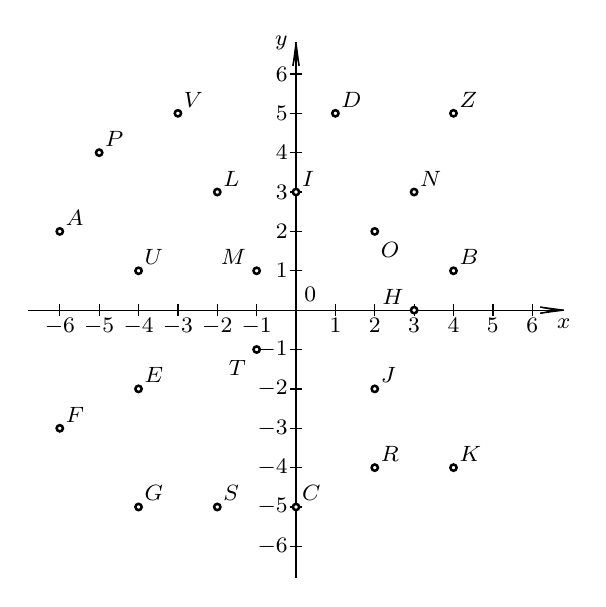
\begin{tikzpicture}
                            % \clip (0,0) rectangle (14.000000,10.000000);
                            {\footnotesize
                            
                            % Drawing 2D Cartesian system
                            \draw (4.000000,4.000000) node [anchor=south west] { $0$ };%
                            \draw [line width=0.016cm] (4.000000,3.925000) -- (4.000000,4.075000);%
                            \draw (4.500000,4.000000) node [anchor=north] { $1$ };%
                            \draw [line width=0.016cm] (4.500000,3.925000) -- (4.500000,4.075000);%
                            \draw (5.000000,4.000000) node [anchor=north] { $2$ };%
                            \draw [line width=0.016cm] (5.000000,3.925000) -- (5.000000,4.075000);%
                            \draw (5.500000,4.000000) node [anchor=north] { $3$ };%
                            \draw [line width=0.016cm] (5.500000,3.925000) -- (5.500000,3.960000);%
                            \draw [line width=0.016cm] (5.500000,4.040000) -- (5.500000,4.075000);%
                            \draw (6.000000,4.000000) node [anchor=north] { $4$ };%
                            \draw [line width=0.016cm] (6.000000,3.925000) -- (6.000000,4.075000);%
                            \draw (6.500000,4.000000) node [anchor=north] { $5$ };%
                            \draw [line width=0.016cm] (6.500000,3.925000) -- (6.500000,4.075000);%
                            \draw (7.000000,4.000000) node [anchor=north] { $6$ };%
                            \draw [line width=0.016cm] (7.000000,3.925000) -- (7.000000,4.075000);%
                            \draw (3.500000,4.000000) node [anchor=north] { $-1$ };%
                            \draw [line width=0.016cm] (3.500000,3.925000) -- (3.500000,4.075000);%
                            \draw (3.000000,4.000000) node [anchor=north] { $-2$ };%
                            \draw [line width=0.016cm] (3.000000,3.925000) -- (3.000000,4.075000);%
                            \draw (2.500000,4.000000) node [anchor=north] { $-3$ };%
                            \draw [line width=0.016cm] (2.500000,3.925000) -- (2.500000,4.075000);%
                            \draw (2.000000,4.000000) node [anchor=north] { $-4$ };%
                            \draw [line width=0.016cm] (2.000000,3.925000) -- (2.000000,4.075000);%
                            \draw (1.500000,4.000000) node [anchor=north] { $-5$ };%
                            \draw [line width=0.016cm] (1.500000,3.925000) -- (1.500000,4.075000);%
                            \draw (1.000000,4.000000) node [anchor=north] { $-6$ };%
                            \draw [line width=0.016cm] (1.000000,3.925000) -- (1.000000,4.075000);%
                            \draw (4.000000,4.500000) node [anchor=east] { $1$ };%
                            \draw [line width=0.016cm] (3.925000,4.500000) -- (4.075000,4.500000);%
                            \draw (4.000000,5.000000) node [anchor=east] { $2$ };%
                            \draw [line width=0.016cm] (3.925000,5.000000) -- (4.075000,5.000000);%
                            \draw (4.000000,5.500000) node [anchor=east] { $3$ };%
                            \draw [line width=0.016cm] (3.925000,5.500000) -- (3.960000,5.500000);%
                            \draw [line width=0.016cm] (4.040000,5.500000) -- (4.075000,5.500000);%
                            \draw (4.000000,6.000000) node [anchor=east] { $4$ };%
                            \draw [line width=0.016cm] (3.925000,6.000000) -- (4.075000,6.000000);%
                            \draw (4.000000,6.500000) node [anchor=east] { $5$ };%
                            \draw [line width=0.016cm] (3.925000,6.500000) -- (4.075000,6.500000);%
                            \draw (4.000000,7.000000) node [anchor=east] { $6$ };%
                            \draw [line width=0.016cm] (3.925000,7.000000) -- (4.075000,7.000000);%
                            \draw (4.000000,3.500000) node [anchor=east] { $-1$ };%
                            \draw [line width=0.016cm] (3.925000,3.500000) -- (4.075000,3.500000);%
                            \draw (4.000000,3.000000) node [anchor=east] { $-2$ };%
                            \draw [line width=0.016cm] (3.925000,3.000000) -- (4.075000,3.000000);%
                            \draw (4.000000,2.500000) node [anchor=east] { $-3$ };%
                            \draw [line width=0.016cm] (3.925000,2.500000) -- (4.075000,2.500000);%
                            \draw (4.000000,2.000000) node [anchor=east] { $-4$ };%
                            \draw [line width=0.016cm] (3.925000,2.000000) -- (4.075000,2.000000);%
                            \draw (4.000000,1.500000) node [anchor=east] { $-5$ };%
                            \draw [line width=0.016cm] (3.925000,1.500000) -- (3.960000,1.500000);%
                            \draw [line width=0.016cm] (4.040000,1.500000) -- (4.075000,1.500000);%
                            \draw (4.000000,1.000000) node [anchor=east] { $-6$ };%
                            \draw [line width=0.016cm] (3.925000,1.000000) -- (4.075000,1.000000);%
                            \draw (7.400000,4.000000) node [anchor=north] { $x$ };%
                            \draw (4.000000,7.400000) node [anchor=east] { $y$ };%
                            \draw [line width=0.016cm] (0.600000,4.000000) -- (5.460000,4.000000);%
                            \draw [line width=0.016cm] (5.540000,4.000000) -- (7.400000,4.000000);%
                            \draw [line width=0.016cm] (7.102567,4.039158) -- (7.400000,4.000000);%
                            \draw [line width=0.016cm] (7.102567,4.039158) -- (7.300000,4.000000);%
                            \draw [line width=0.016cm] (7.102567,3.960842) -- (7.400000,4.000000);%
                            \draw [line width=0.016cm] (7.102567,3.960842) -- (7.300000,4.000000);%
                            \draw [line width=0.016cm] (4.000000,0.600000) -- (4.000000,1.460000);%
                            \draw [line width=0.016cm] (4.000000,1.540000) -- (4.000000,5.460000);%
                            \draw [line width=0.016cm] (4.000000,5.540000) -- (4.000000,7.400000);%
                            \draw [line width=0.016cm] (3.960842,7.102567) -- (4.000000,7.400000);%
                            \draw [line width=0.016cm] (3.960842,7.102567) -- (4.000000,7.300000);%
                            \draw [line width=0.016cm] (4.039158,7.102567) -- (4.000000,7.400000);%
                            \draw [line width=0.016cm] (4.039158,7.102567) -- (4.000000,7.300000);%
                            
                            % Marking point A by circle
                            \draw [line width=0.032cm] (1.000000,5.000000) circle (0.040000);%
                            \draw (0.970000,4.970000) node [anchor=south west] { $A$ };%
                            
                            % Marking point B by circle
                            \draw [line width=0.032cm] (6.000000,4.500000) circle (0.040000);%
                            \draw (5.970000,4.470000) node [anchor=south west] { $B$ };%
                            
                            % Marking point C by circle
                            \draw [line width=0.032cm] (4.000000,1.500000) circle (0.040000);%
                            \draw (3.970000,1.470000) node [anchor=south west] { $C$ };%
                            
                            % Marking point D by circle
                            \draw [line width=0.032cm] (4.500000,6.500000) circle (0.040000);%
                            \draw (4.470000,6.470000) node [anchor=south west] { $D$ };%
                            
                            % Marking point E by circle
                            \draw [line width=0.032cm] (2.000000,3.000000) circle (0.040000);%
                            \draw (1.970000,2.970000) node [anchor=south west] { $E$ };%
                            
                            % Marking point F by circle
                            \draw [line width=0.032cm] (1.000000,2.500000) circle (0.040000);%
                            \draw (0.970000,2.470000) node [anchor=south west] { $F$ };%
                            
                            % Marking point G by circle
                            \draw [line width=0.032cm] (2.000000,1.500000) circle (0.040000);%
                            \draw (1.970000,1.470000) node [anchor=south west] { $G$ };%
                            
                            % Marking point H by circle
                            \draw [line width=0.032cm] (5.500000,4.000000) circle (0.040000);%
                            \draw (5.470000,3.970000) node [anchor=south east] { $H$ };%
                            
                            % Marking point I by circle
                            \draw [line width=0.032cm] (4.000000,5.500000) circle (0.040000);%
                            \draw (3.970000,5.470000) node [anchor=south west] { $I$ };%
                            
                            % Marking point J by circle
                            \draw [line width=0.032cm] (5.000000,3.000000) circle (0.040000);%
                            \draw (4.970000,2.970000) node [anchor=south west] { $J$ };%
                            
                            % Marking point K by circle
                            \draw [line width=0.032cm] (6.000000,2.000000) circle (0.040000);%
                            \draw (5.970000,1.970000) node [anchor=south west] { $K$ };%
                            
                            % Marking point L by circle
                            \draw [line width=0.032cm] (3.000000,5.500000) circle (0.040000);%
                            \draw (2.970000,5.470000) node [anchor=south west] { $L$ };%
                            
                            % Marking point M by circle
                            \draw [line width=0.032cm] (3.500000,4.500000) circle (0.040000);%
                            \draw (3.470000,4.470000) node [anchor=south east] { $M$ };%
                            
                            % Marking point N by circle
                            \draw [line width=0.032cm] (5.500000,5.500000) circle (0.040000);%
                            \draw (5.470000,5.470000) node [anchor=south west] { $N$ };%
                            
                            % Marking point O by circle
                            \draw [line width=0.032cm] (5.000000,5.000000) circle (0.040000);%
                            \draw (4.970000,4.970000) node [anchor=north west] { $O$ };%
                            
                            % Marking point P by circle
                            \draw [line width=0.032cm] (1.500000,6.000000) circle (0.040000);%
                            \draw (1.470000,5.970000) node [anchor=south west] { $P$ };%
                            
                            % Marking point R by circle
                            \draw [line width=0.032cm] (5.000000,2.000000) circle (0.040000);%
                            \draw (4.970000,1.970000) node [anchor=south west] { $R$ };%
                            
                            % Marking point S by circle
                            \draw [line width=0.032cm] (3.000000,1.500000) circle (0.040000);%
                            \draw (2.970000,1.470000) node [anchor=south west] { $S$ };%
                            
                            % Marking point T by circle
                            \draw [line width=0.032cm] (3.500000,3.500000) circle (0.040000);%
                            \draw (3.470000,3.470000) node [anchor=north east] { $T$ };%
                            
                            % Marking point U by circle
                            \draw [line width=0.032cm] (2.000000,4.500000) circle (0.040000);%
                            \draw (1.970000,4.470000) node [anchor=south west] { $U$ };%
                            
                            % Marking point V by circle
                            \draw [line width=0.032cm] (2.500000,6.500000) circle (0.040000);%
                            \draw (2.470000,6.470000) node [anchor=south west] { $V$ };%
                            
                            % Marking point Z by circle
                            \draw [line width=0.032cm] (6.000000,6.500000) circle (0.040000);%
                            \draw (5.970000,6.470000) node [anchor=south west] { $Z$ };%
                            }
                        \end{tikzpicture}
                            
                    \end{figure}

                
                \end{columns}

            \end{exampleblock}}

            

        \end{frame}


        \begin{frame}
            \only<2->{\begin{exampleblock}{Naloga}
                Narišite množico točk.
                \vskip-1.2em
                \begin{columns}
                    \column{0.5\textwidth}
                    \begin{itemize}
                        \item $\left\{T(x,y);~x\geq -1\right\}$
                        \item $\left\{T(x,y);~y\leq 3\right\}$
                        \item $\left\{T(x,y);~x\leq 4 \land y<-1\right\}$
                        \item $\left\{T(x,y);~x\geq -2 \land y<1\right\}$
                        \item $\left\{T(x,y);~-2<x\leq 4\land -3<y<1 \right\}$
                        \item $\left\{T(x,y);~ 0\leq x<4 \land -3\leq y<3\right\}$
                        \item $\left\{T(x,y);~ x<4\land y<-1\right\}$
                    \end{itemize}

                    \column{0.47\textwidth}
                    \begin{itemize}
                        \item $\left\{T(x,y);~ \left|x\right|<3\right\}$
                        \item $\left\{T(x,y);~ x\geq 1 \land \left|y\right|<1\right\}$
                        \item $\left\{T(x,y);~ \left|x-3\right|<1 \land y\geq 1\right\}$
                        \item $\left\{T(x,y);~ \left|x\right|<2 \land \left|y+3\right|\leq 1\right\}$
                        \item $\left\{T(x,y);~ x=y\right\}$
                        \item $\left\{T(x,y);~ x\geq y\right\}$
                        \item $\left\{T(x,y);~ xy\geq 0\right\}$
                    \end{itemize}
                \end{columns}

            \end{exampleblock}}
        \end{frame}


        \begin{frame}

            \only<2->{\begin{exampleblock}{Naloga}
                Zapišite množico točk, ki je upodobljena v koordinatnem sistemu.

                \begin{columns}
                    \column{0.48\textwidth}
                    \vskip-1.5em
                    \begin{figure}[H]
                        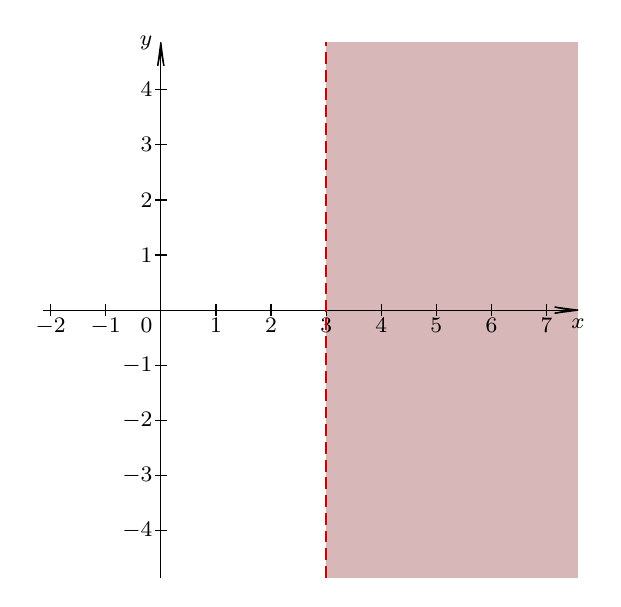
\begin{tikzpicture}
                            % \clip (0,0) rectangle (14.000000,10.000000);
                            {\footnotesize
                                                        
                            % Changing color 215 183 183
                            \definecolor{r215g183b183}{rgb}{0.843137,0.717647,0.717647}%
                            \color{r215g183b183}% 
                            
                            % Filling rectangle left-bottom: X right-top: Y
                            \fill (4.200000,0.600000) -- (7.400000,0.600000) -- (7.400000,7.400000) -- (4.200000,7.400000);%
                            
                            % Changing color 0 0 0
                            \definecolor{r0g0b0}{rgb}{0.000000,0.000000,0.000000}%
                            \color{r0g0b0}% 
                            
                            % Drawing 2D Cartesian system
                            \draw (2.100000,4.000000) node [anchor=north east] { $0$ };%
                            \draw [line width=0.016cm] (2.100000,3.925000) -- (2.100000,4.075000);%
                            \draw (2.800000,4.000000) node [anchor=north] { $1$ };%
                            \draw [line width=0.016cm] (2.800000,3.925000) -- (2.800000,4.075000);%
                            \draw (3.500000,4.000000) node [anchor=north] { $2$ };%
                            \draw [line width=0.016cm] (3.500000,3.925000) -- (3.500000,4.075000);%
                            \draw (4.200000,4.000000) node [anchor=north] { $3$ };%
                            \draw [line width=0.016cm] (4.200000,3.925000) -- (4.200000,4.075000);%
                            \draw (4.900000,4.000000) node [anchor=north] { $4$ };%
                            \draw [line width=0.016cm] (4.900000,3.925000) -- (4.900000,4.075000);%
                            \draw (5.600000,4.000000) node [anchor=north] { $5$ };%
                            \draw [line width=0.016cm] (5.600000,3.925000) -- (5.600000,4.075000);%
                            \draw (6.300000,4.000000) node [anchor=north] { $6$ };%
                            \draw [line width=0.016cm] (6.300000,3.925000) -- (6.300000,4.075000);%
                            \draw (7.000000,4.000000) node [anchor=north] { $7$ };%
                            \draw [line width=0.016cm] (7.000000,3.925000) -- (7.000000,4.075000);%
                            \draw (1.400000,4.000000) node [anchor=north] { $-1$ };%
                            \draw [line width=0.016cm] (1.400000,3.925000) -- (1.400000,4.075000);%
                            \draw (0.700000,4.000000) node [anchor=north] { $-2$ };%
                            \draw [line width=0.016cm] (0.700000,3.925000) -- (0.700000,4.075000);%
                            \draw (2.100000,4.700000) node [anchor=east] { $1$ };%
                            \draw [line width=0.016cm] (2.025000,4.700000) -- (2.175000,4.700000);%
                            \draw (2.100000,5.400000) node [anchor=east] { $2$ };%
                            \draw [line width=0.016cm] (2.025000,5.400000) -- (2.175000,5.400000);%
                            \draw (2.100000,6.100000) node [anchor=east] { $3$ };%
                            \draw [line width=0.016cm] (2.025000,6.100000) -- (2.175000,6.100000);%
                            \draw (2.100000,6.800000) node [anchor=east] { $4$ };%
                            \draw [line width=0.016cm] (2.025000,6.800000) -- (2.175000,6.800000);%
                            \draw (2.100000,3.300000) node [anchor=east] { $-1$ };%
                            \draw [line width=0.016cm] (2.025000,3.300000) -- (2.175000,3.300000);%
                            \draw (2.100000,2.600000) node [anchor=east] { $-2$ };%
                            \draw [line width=0.016cm] (2.025000,2.600000) -- (2.175000,2.600000);%
                            \draw (2.100000,1.900000) node [anchor=east] { $-3$ };%
                            \draw [line width=0.016cm] (2.025000,1.900000) -- (2.175000,1.900000);%
                            \draw (2.100000,1.200000) node [anchor=east] { $-4$ };%
                            \draw [line width=0.016cm] (2.025000,1.200000) -- (2.175000,1.200000);%
                            \draw (7.400000,4.000000) node [anchor=north] { $x$ };%
                            \draw (2.100000,7.400000) node [anchor=east] { $y$ };%
                            \draw [line width=0.016cm] (0.600000,4.000000) -- (7.400000,4.000000);%
                            \draw [line width=0.016cm] (7.102567,4.039158) -- (7.400000,4.000000);%
                            \draw [line width=0.016cm] (7.102567,4.039158) -- (7.300000,4.000000);%
                            \draw [line width=0.016cm] (7.102567,3.960842) -- (7.400000,4.000000);%
                            \draw [line width=0.016cm] (7.102567,3.960842) -- (7.300000,4.000000);%
                            \draw [line width=0.016cm] (2.100000,0.600000) -- (2.100000,7.400000);%
                            \draw [line width=0.016cm] (2.060842,7.102567) -- (2.100000,7.400000);%
                            \draw [line width=0.016cm] (2.060842,7.102567) -- (2.100000,7.300000);%
                            \draw [line width=0.016cm] (2.139158,7.102567) -- (2.100000,7.400000);%
                            \draw [line width=0.016cm] (2.139158,7.102567) -- (2.100000,7.300000);%
                            
                            % Changing color 204 0 0
                            \definecolor{r204g0b0}{rgb}{0.800000,0.000000,0.000000}%
                            \color{r204g0b0}% 
                            
                            % Drawing line A B
                            \draw [line width=0.032cm] (4.200000,0.600000) -- (4.200000,0.750000);%
                            \draw [line width=0.032cm] (4.200000,0.825000) -- (4.200000,0.975000);%
                            \draw [line width=0.032cm] (4.200000,1.050000) -- (4.200000,1.200000);%
                            \draw [line width=0.032cm] (4.200000,1.275000) -- (4.200000,1.425000);%
                            \draw [line width=0.032cm] (4.200000,1.500000) -- (4.200000,1.650000);%
                            \draw [line width=0.032cm] (4.200000,1.725000) -- (4.200000,1.875000);%
                            \draw [line width=0.032cm] (4.200000,1.950000) -- (4.200000,2.100000);%
                            \draw [line width=0.032cm] (4.200000,2.175000) -- (4.200000,2.325000);%
                            \draw [line width=0.032cm] (4.200000,2.400000) -- (4.200000,2.550000);%
                            \draw [line width=0.032cm] (4.200000,2.625000) -- (4.200000,2.775000);%
                            \draw [line width=0.032cm] (4.200000,2.850000) -- (4.200000,3.000000);%
                            \draw [line width=0.032cm] (4.200000,3.075000) -- (4.200000,3.225000);%
                            \draw [line width=0.032cm] (4.200000,3.300000) -- (4.200000,3.450000);%
                            \draw [line width=0.032cm] (4.200000,3.525000) -- (4.200000,3.675000);%
                            \draw [line width=0.032cm] (4.200000,3.750000) -- (4.200000,3.900000);%
                            \draw [line width=0.032cm] (4.200000,3.975000) -- (4.200000,4.125000);%
                            \draw [line width=0.032cm] (4.200000,4.200000) -- (4.200000,4.350000);%
                            \draw [line width=0.032cm] (4.200000,4.425000) -- (4.200000,4.575000);%
                            \draw [line width=0.032cm] (4.200000,4.650000) -- (4.200000,4.800000);%
                            \draw [line width=0.032cm] (4.200000,4.875000) -- (4.200000,5.025000);%
                            \draw [line width=0.032cm] (4.200000,5.100000) -- (4.200000,5.250000);%
                            \draw [line width=0.032cm] (4.200000,5.325000) -- (4.200000,5.475000);%
                            \draw [line width=0.032cm] (4.200000,5.550000) -- (4.200000,5.700000);%
                            \draw [line width=0.032cm] (4.200000,5.775000) -- (4.200000,5.925000);%
                            \draw [line width=0.032cm] (4.200000,6.000000) -- (4.200000,6.150000);%
                            \draw [line width=0.032cm] (4.200000,6.225000) -- (4.200000,6.375000);%
                            \draw [line width=0.032cm] (4.200000,6.450000) -- (4.200000,6.600000);%
                            \draw [line width=0.032cm] (4.200000,6.675000) -- (4.200000,6.825000);%
                            \draw [line width=0.032cm] (4.200000,6.900000) -- (4.200000,7.050000);%
                            \draw [line width=0.032cm] (4.200000,7.125000) -- (4.200000,7.275000);%
                            \draw [line width=0.032cm] (4.200000,7.350000) -- (4.200000,7.400000);%
                            \color{black}
                            }
                        \end{tikzpicture}
                            
                    \end{figure}

                    \column{0.48\textwidth}
                    \vskip-1.5em
                    \begin{figure}[H]
                        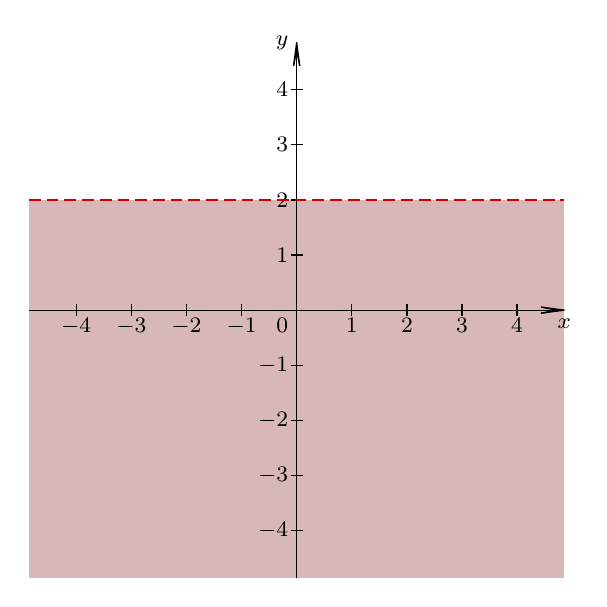
\begin{tikzpicture}
                            % \clip (0,0) rectangle (14.000000,10.000000);
                            {\footnotesize
                                                        
                            % Changing color 215 183 183
                            \definecolor{r215g183b183}{rgb}{0.843137,0.717647,0.717647}%
                            \color{r215g183b183}% 
                            
                            % Filling rectangle left-bottom: X right-top: Y
                            \fill (0.600000,0.600000) -- (7.400000,0.600000) -- (7.400000,5.400000) -- (0.600000,5.400000);%
                            
                            % Changing color 0 0 0
                            \definecolor{r0g0b0}{rgb}{0.000000,0.000000,0.000000}%
                            \color{r0g0b0}% 
                            
                            % Drawing 2D Cartesian system
                            \draw (4.000000,4.000000) node [anchor=north east] { $0$ };%
                            \draw [line width=0.016cm] (4.000000,3.925000) -- (4.000000,4.075000);%
                            \draw (4.700000,4.000000) node [anchor=north] { $1$ };%
                            \draw [line width=0.016cm] (4.700000,3.925000) -- (4.700000,4.075000);%
                            \draw (5.400000,4.000000) node [anchor=north] { $2$ };%
                            \draw [line width=0.016cm] (5.400000,3.925000) -- (5.400000,4.075000);%
                            \draw (6.100000,4.000000) node [anchor=north] { $3$ };%
                            \draw [line width=0.016cm] (6.100000,3.925000) -- (6.100000,4.075000);%
                            \draw (6.800000,4.000000) node [anchor=north] { $4$ };%
                            \draw [line width=0.016cm] (6.800000,3.925000) -- (6.800000,4.075000);%
                            \draw (3.300000,4.000000) node [anchor=north] { $-1$ };%
                            \draw [line width=0.016cm] (3.300000,3.925000) -- (3.300000,4.075000);%
                            \draw (2.600000,4.000000) node [anchor=north] { $-2$ };%
                            \draw [line width=0.016cm] (2.600000,3.925000) -- (2.600000,4.075000);%
                            \draw (1.900000,4.000000) node [anchor=north] { $-3$ };%
                            \draw [line width=0.016cm] (1.900000,3.925000) -- (1.900000,4.075000);%
                            \draw (1.200000,4.000000) node [anchor=north] { $-4$ };%
                            \draw [line width=0.016cm] (1.200000,3.925000) -- (1.200000,4.075000);%
                            \draw (4.000000,4.700000) node [anchor=east] { $1$ };%
                            \draw [line width=0.016cm] (3.925000,4.700000) -- (4.075000,4.700000);%
                            \draw (4.000000,5.400000) node [anchor=east] { $2$ };%
                            \draw [line width=0.016cm] (3.925000,5.400000) -- (4.075000,5.400000);%
                            \draw (4.000000,6.100000) node [anchor=east] { $3$ };%
                            \draw [line width=0.016cm] (3.925000,6.100000) -- (4.075000,6.100000);%
                            \draw (4.000000,6.800000) node [anchor=east] { $4$ };%
                            \draw [line width=0.016cm] (3.925000,6.800000) -- (4.075000,6.800000);%
                            \draw (4.000000,3.300000) node [anchor=east] { $-1$ };%
                            \draw [line width=0.016cm] (3.925000,3.300000) -- (4.075000,3.300000);%
                            \draw (4.000000,2.600000) node [anchor=east] { $-2$ };%
                            \draw [line width=0.016cm] (3.925000,2.600000) -- (4.075000,2.600000);%
                            \draw (4.000000,1.900000) node [anchor=east] { $-3$ };%
                            \draw [line width=0.016cm] (3.925000,1.900000) -- (4.075000,1.900000);%
                            \draw (4.000000,1.200000) node [anchor=east] { $-4$ };%
                            \draw [line width=0.016cm] (3.925000,1.200000) -- (4.075000,1.200000);%
                            \draw (7.400000,4.000000) node [anchor=north] { $x$ };%
                            \draw (4.000000,7.400000) node [anchor=east] { $y$ };%
                            \draw [line width=0.016cm] (0.600000,4.000000) -- (7.400000,4.000000);%
                            \draw [line width=0.016cm] (7.102567,4.039158) -- (7.400000,4.000000);%
                            \draw [line width=0.016cm] (7.102567,4.039158) -- (7.300000,4.000000);%
                            \draw [line width=0.016cm] (7.102567,3.960842) -- (7.400000,4.000000);%
                            \draw [line width=0.016cm] (7.102567,3.960842) -- (7.300000,4.000000);%
                            \draw [line width=0.016cm] (4.000000,0.600000) -- (4.000000,7.400000);%
                            \draw [line width=0.016cm] (3.960842,7.102567) -- (4.000000,7.400000);%
                            \draw [line width=0.016cm] (3.960842,7.102567) -- (4.000000,7.300000);%
                            \draw [line width=0.016cm] (4.039158,7.102567) -- (4.000000,7.400000);%
                            \draw [line width=0.016cm] (4.039158,7.102567) -- (4.000000,7.300000);%
                            
                            % Changing color 204 0 0
                            \definecolor{r204g0b0}{rgb}{0.800000,0.000000,0.000000}%
                            \color{r204g0b0}% 
                            
                            % Drawing line A B
                            \draw [line width=0.032cm] (0.600000,5.400000) -- (0.750000,5.400000);%
                            \draw [line width=0.032cm] (0.825000,5.400000) -- (0.975000,5.400000);%
                            \draw [line width=0.032cm] (1.050000,5.400000) -- (1.200000,5.400000);%
                            \draw [line width=0.032cm] (1.275000,5.400000) -- (1.425000,5.400000);%
                            \draw [line width=0.032cm] (1.500000,5.400000) -- (1.650000,5.400000);%
                            \draw [line width=0.032cm] (1.725000,5.400000) -- (1.875000,5.400000);%
                            \draw [line width=0.032cm] (1.950000,5.400000) -- (2.100000,5.400000);%
                            \draw [line width=0.032cm] (2.175000,5.400000) -- (2.325000,5.400000);%
                            \draw [line width=0.032cm] (2.400000,5.400000) -- (2.550000,5.400000);%
                            \draw [line width=0.032cm] (2.625000,5.400000) -- (2.775000,5.400000);%
                            \draw [line width=0.032cm] (2.850000,5.400000) -- (3.000000,5.400000);%
                            \draw [line width=0.032cm] (3.075000,5.400000) -- (3.225000,5.400000);%
                            \draw [line width=0.032cm] (3.300000,5.400000) -- (3.450000,5.400000);%
                            \draw [line width=0.032cm] (3.525000,5.400000) -- (3.675000,5.400000);%
                            \draw [line width=0.032cm] (3.750000,5.400000) -- (3.900000,5.400000);%
                            \draw [line width=0.032cm] (3.975000,5.400000) -- (4.125000,5.400000);%
                            \draw [line width=0.032cm] (4.200000,5.400000) -- (4.350000,5.400000);%
                            \draw [line width=0.032cm] (4.425000,5.400000) -- (4.575000,5.400000);%
                            \draw [line width=0.032cm] (4.650000,5.400000) -- (4.800000,5.400000);%
                            \draw [line width=0.032cm] (4.875000,5.400000) -- (5.025000,5.400000);%
                            \draw [line width=0.032cm] (5.100000,5.400000) -- (5.250000,5.400000);%
                            \draw [line width=0.032cm] (5.325000,5.400000) -- (5.475000,5.400000);%
                            \draw [line width=0.032cm] (5.550000,5.400000) -- (5.700000,5.400000);%
                            \draw [line width=0.032cm] (5.775000,5.400000) -- (5.925000,5.400000);%
                            \draw [line width=0.032cm] (6.000000,5.400000) -- (6.150000,5.400000);%
                            \draw [line width=0.032cm] (6.225000,5.400000) -- (6.375000,5.400000);%
                            \draw [line width=0.032cm] (6.450000,5.400000) -- (6.600000,5.400000);%
                            \draw [line width=0.032cm] (6.675000,5.400000) -- (6.825000,5.400000);%
                            \draw [line width=0.032cm] (6.900000,5.400000) -- (7.050000,5.400000);%
                            \draw [line width=0.032cm] (7.125000,5.400000) -- (7.275000,5.400000);%
                            \draw [line width=0.032cm] (7.350000,5.400000) -- (7.400000,5.400000);%
                            \color{black}
                            }
                        \end{tikzpicture}
                            
                    \end{figure}

                \end{columns}
            \end{exampleblock}}

        \end{frame}


        \begin{frame}

            \only<2->{\begin{exampleblock}{}

                \begin{columns}
                    \column{0.48\textwidth}
                    \vskip-1.5em
                    \begin{figure}[H]
                        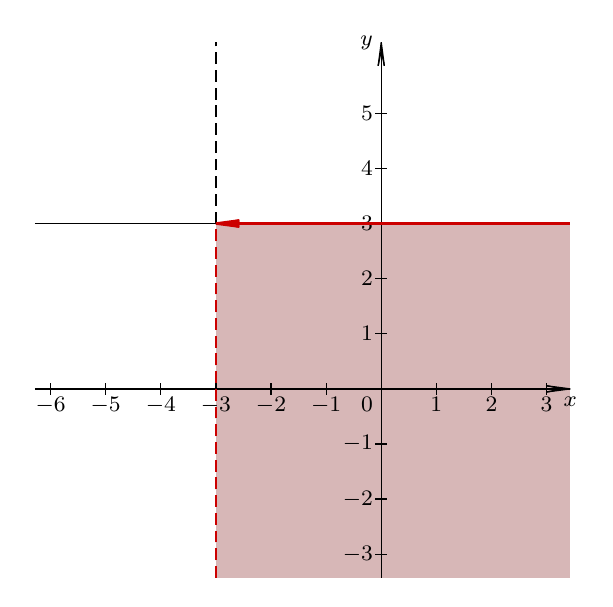
\begin{tikzpicture}
                            % \clip (0,0) rectangle (14.000000,10.000000);
                            {\footnotesize
                                                   
                            % Changing color 215 183 183
                            \definecolor{r215g183b183}{rgb}{0.843137,0.717647,0.717647}%
                            \color{r215g183b183}% 
                            
                            % Filling rectangle left-bottom: X right-top: Y
                            \fill (2.900000,0.600000) -- (7.400000,0.600000) -- (7.400000,5.100000) -- (2.900000,5.100000);%
                            
                            % Changing color 0 0 0
                            \definecolor{r0g0b0}{rgb}{0.000000,0.000000,0.000000}%
                            \color{r0g0b0}% 
                            
                            % Drawing 2D Cartesian system
                            \draw (5.000000,3.000000) node [anchor=north east] { $0$ };%
                            \draw [line width=0.016cm] (5.000000,2.925000) -- (5.000000,3.075000);%
                            \draw (5.700000,3.000000) node [anchor=north] { $1$ };%
                            \draw [line width=0.016cm] (5.700000,2.925000) -- (5.700000,3.075000);%
                            \draw (6.400000,3.000000) node [anchor=north] { $2$ };%
                            \draw [line width=0.016cm] (6.400000,2.925000) -- (6.400000,3.075000);%
                            \draw (7.100000,3.000000) node [anchor=north] { $3$ };%
                            \draw [line width=0.016cm] (7.100000,2.925000) -- (7.100000,3.075000);%
                            \draw (4.300000,3.000000) node [anchor=north] { $-1$ };%
                            \draw [line width=0.016cm] (4.300000,2.925000) -- (4.300000,3.075000);%
                            \draw (3.600000,3.000000) node [anchor=north] { $-2$ };%
                            \draw [line width=0.016cm] (3.600000,2.925000) -- (3.600000,3.075000);%
                            \draw (2.900000,3.000000) node [anchor=north] { $-3$ };%
                            \draw [line width=0.016cm] (2.900000,2.925000) -- (2.900000,3.075000);%
                            \draw (2.200000,3.000000) node [anchor=north] { $-4$ };%
                            \draw [line width=0.016cm] (2.200000,2.925000) -- (2.200000,3.075000);%
                            \draw (1.500000,3.000000) node [anchor=north] { $-5$ };%
                            \draw [line width=0.016cm] (1.500000,2.925000) -- (1.500000,3.075000);%
                            \draw (0.800000,3.000000) node [anchor=north] { $-6$ };%
                            \draw [line width=0.016cm] (0.800000,2.925000) -- (0.800000,3.075000);%
                            \draw (5.000000,3.700000) node [anchor=east] { $1$ };%
                            \draw [line width=0.016cm] (4.925000,3.700000) -- (5.075000,3.700000);%
                            \draw (5.000000,4.400000) node [anchor=east] { $2$ };%
                            \draw [line width=0.016cm] (4.925000,4.400000) -- (5.075000,4.400000);%
                            \draw (5.000000,5.100000) node [anchor=east] { $3$ };%
                            \draw [line width=0.016cm] (4.925000,5.100000) -- (5.075000,5.100000);%
                            \draw (5.000000,5.800000) node [anchor=east] { $4$ };%
                            \draw [line width=0.016cm] (4.925000,5.800000) -- (5.075000,5.800000);%
                            \draw (5.000000,6.500000) node [anchor=east] { $5$ };%
                            \draw [line width=0.016cm] (4.925000,6.500000) -- (5.075000,6.500000);%
                            % \draw (5.000000,7.200000) node [anchor=east] { $6$ };%
                            % \draw [line width=0.016cm] (4.925000,7.200000) -- (5.075000,7.200000);%
                            \draw (5.000000,2.300000) node [anchor=east] { $-1$ };%
                            \draw [line width=0.016cm] (4.925000,2.300000) -- (5.075000,2.300000);%
                            \draw (5.000000,1.600000) node [anchor=east] { $-2$ };%
                            \draw [line width=0.016cm] (4.925000,1.600000) -- (5.075000,1.600000);%
                            \draw (5.000000,0.900000) node [anchor=east] { $-3$ };%
                            \draw [line width=0.016cm] (4.925000,0.900000) -- (5.075000,0.900000);%
                            \draw (7.400000,3.000000) node [anchor=north] { $x$ };%
                            \draw (5.000000,7.400000) node [anchor=east] { $y$ };%
                            \draw [line width=0.016cm] (0.600000,3.000000) -- (7.400000,3.000000);%
                            \draw [line width=0.016cm] (7.102567,3.039158) -- (7.400000,3.000000);%
                            \draw [line width=0.016cm] (7.102567,3.039158) -- (7.300000,3.000000);%
                            \draw [line width=0.016cm] (7.102567,2.960842) -- (7.400000,3.000000);%
                            \draw [line width=0.016cm] (7.102567,2.960842) -- (7.300000,3.000000);%
                            \draw [line width=0.016cm] (5.000000,0.600000) -- (5.000000,7.400000);%
                            \draw [line width=0.016cm] (4.960842,7.102567) -- (5.000000,7.400000);%
                            \draw [line width=0.016cm] (4.960842,7.102567) -- (5.000000,7.300000);%
                            \draw [line width=0.016cm] (5.039158,7.102567) -- (5.000000,7.400000);%
                            \draw [line width=0.016cm] (5.039158,7.102567) -- (5.000000,7.300000);%
                            
                            % Drawing line A B
                            \draw [line width=0.016cm] (2.900000,0.600000) -- (2.900000,0.750000);%
                            \draw [line width=0.016cm] (2.900000,0.825000) -- (2.900000,0.975000);%
                            \draw [line width=0.016cm] (2.900000,1.050000) -- (2.900000,1.200000);%
                            \draw [line width=0.016cm] (2.900000,1.275000) -- (2.900000,1.425000);%
                            \draw [line width=0.016cm] (2.900000,1.500000) -- (2.900000,1.650000);%
                            \draw [line width=0.016cm] (2.900000,1.725000) -- (2.900000,1.875000);%
                            \draw [line width=0.016cm] (2.900000,1.950000) -- (2.900000,2.100000);%
                            \draw [line width=0.016cm] (2.900000,2.175000) -- (2.900000,2.325000);%
                            \draw [line width=0.016cm] (2.900000,2.400000) -- (2.900000,2.550000);%
                            \draw [line width=0.016cm] (2.900000,2.625000) -- (2.900000,2.775000);%
                            \draw [line width=0.016cm] (2.900000,2.850000) -- (2.900000,3.000000);%
                            \draw [line width=0.016cm] (2.900000,3.075000) -- (2.900000,3.225000);%
                            \draw [line width=0.016cm] (2.900000,3.300000) -- (2.900000,3.450000);%
                            \draw [line width=0.016cm] (2.900000,3.525000) -- (2.900000,3.675000);%
                            \draw [line width=0.016cm] (2.900000,3.750000) -- (2.900000,3.900000);%
                            \draw [line width=0.016cm] (2.900000,3.975000) -- (2.900000,4.125000);%
                            \draw [line width=0.016cm] (2.900000,4.200000) -- (2.900000,4.350000);%
                            \draw [line width=0.016cm] (2.900000,4.425000) -- (2.900000,4.575000);%
                            \draw [line width=0.016cm] (2.900000,4.650000) -- (2.900000,4.800000);%
                            \draw [line width=0.016cm] (2.900000,4.875000) -- (2.900000,5.025000);%
                            \draw [line width=0.016cm] (2.900000,5.100000) -- (2.900000,5.250000);%
                            \draw [line width=0.016cm] (2.900000,5.325000) -- (2.900000,5.475000);%
                            \draw [line width=0.016cm] (2.900000,5.550000) -- (2.900000,5.700000);%
                            \draw [line width=0.016cm] (2.900000,5.775000) -- (2.900000,5.925000);%
                            \draw [line width=0.016cm] (2.900000,6.000000) -- (2.900000,6.150000);%
                            \draw [line width=0.016cm] (2.900000,6.225000) -- (2.900000,6.375000);%
                            \draw [line width=0.016cm] (2.900000,6.450000) -- (2.900000,6.600000);%
                            \draw [line width=0.016cm] (2.900000,6.675000) -- (2.900000,6.825000);%
                            \draw [line width=0.016cm] (2.900000,6.900000) -- (2.900000,7.050000);%
                            \draw [line width=0.016cm] (2.900000,7.125000) -- (2.900000,7.275000);%
                            \draw [line width=0.016cm] (2.900000,7.350000) -- (2.900000,7.400000);%
                            
                            % Drawing line C D
                            \draw [line width=0.016cm] (0.600000,5.100000) -- (7.400000,5.100000);%
                            
                            % Changing color 204 0 0
                            \definecolor{r204g0b0}{rgb}{0.800000,0.000000,0.000000}%
                            \color{r204g0b0}% 
                            
                            % Drawing segment A B
                            \draw [line width=0.032cm] (2.900000,0.600000) -- (2.900000,0.750000);%
                            \draw [line width=0.032cm] (2.900000,0.825000) -- (2.900000,0.975000);%
                            \draw [line width=0.032cm] (2.900000,1.050000) -- (2.900000,1.200000);%
                            \draw [line width=0.032cm] (2.900000,1.275000) -- (2.900000,1.425000);%
                            \draw [line width=0.032cm] (2.900000,1.500000) -- (2.900000,1.650000);%
                            \draw [line width=0.032cm] (2.900000,1.725000) -- (2.900000,1.875000);%
                            \draw [line width=0.032cm] (2.900000,1.950000) -- (2.900000,2.100000);%
                            \draw [line width=0.032cm] (2.900000,2.175000) -- (2.900000,2.325000);%
                            \draw [line width=0.032cm] (2.900000,2.400000) -- (2.900000,2.550000);%
                            \draw [line width=0.032cm] (2.900000,2.625000) -- (2.900000,2.775000);%
                            \draw [line width=0.032cm] (2.900000,2.850000) -- (2.900000,3.000000);%
                            \draw [line width=0.032cm] (2.900000,3.075000) -- (2.900000,3.225000);%
                            \draw [line width=0.032cm] (2.900000,3.300000) -- (2.900000,3.450000);%
                            \draw [line width=0.032cm] (2.900000,3.525000) -- (2.900000,3.675000);%
                            \draw [line width=0.032cm] (2.900000,3.750000) -- (2.900000,3.900000);%
                            \draw [line width=0.032cm] (2.900000,3.975000) -- (2.900000,4.125000);%
                            \draw [line width=0.032cm] (2.900000,4.200000) -- (2.900000,4.350000);%
                            \draw [line width=0.032cm] (2.900000,4.425000) -- (2.900000,4.575000);%
                            \draw [line width=0.032cm] (2.900000,4.650000) -- (2.900000,4.800000);%
                            \draw [line width=0.032cm] (2.900000,4.875000) -- (2.900000,5.025000);%
                            
                            % Drawing segment C D
                            \draw [line width=0.032cm] (2.900000,5.100000) -- (7.400000,5.100000);%
                            
                            % Drawing arrow D C 1.00
                            \draw [line width=0.032cm] (3.197433,5.060842) -- (2.900000,5.100000);%
                            \draw [line width=0.032cm] (3.197433,5.060842) -- (2.999144,5.100000);%
                            \draw [line width=0.032cm] (3.197433,5.139158) -- (2.900000,5.100000);%
                            \draw [line width=0.032cm] (3.197433,5.139158) -- (2.999144,5.100000);%
                            \color{black}
                            }
                        \end{tikzpicture}
                            
                    \end{figure}

                    \column{0.48\textwidth}
                    \vskip-1.5em
                    \begin{figure}[H]
                        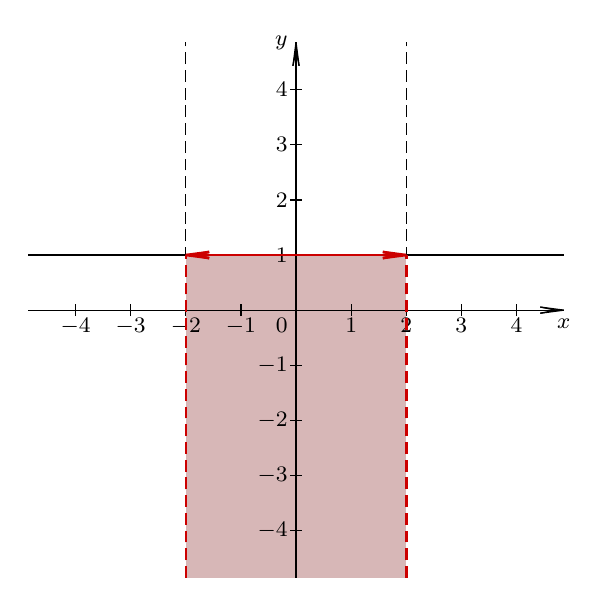
\begin{tikzpicture}
                            % \clip (0,0) rectangle (14.000000,10.000000);
                            {\footnotesize
                                                        
                            % Changing color 215 183 183
                            \definecolor{r215g183b183}{rgb}{0.843137,0.717647,0.717647}%
                            \color{r215g183b183}% 
                            
                            % Filling rectangle left-bottom: X right-top: Y
                            \fill (2.600000,0.600000) -- (5.400000,0.600000) -- (5.400000,4.700000) -- (2.600000,4.700000);%
                            
                            % Changing color 0 0 0
                            \definecolor{r0g0b0}{rgb}{0.000000,0.000000,0.000000}%
                            \color{r0g0b0}% 
                            
                            % Drawing 2D Cartesian system
                            \draw (4.000000,4.000000) node [anchor=north east] { $0$ };%
                            \draw [line width=0.016cm] (4.000000,3.925000) -- (4.000000,4.075000);%
                            \draw (4.700000,4.000000) node [anchor=north] { $1$ };%
                            \draw [line width=0.016cm] (4.700000,3.925000) -- (4.700000,4.075000);%
                            \draw (5.400000,4.000000) node [anchor=north] { $2$ };%
                            \draw [line width=0.016cm] (5.400000,3.925000) -- (5.400000,4.075000);%
                            \draw (6.100000,4.000000) node [anchor=north] { $3$ };%
                            \draw [line width=0.016cm] (6.100000,3.925000) -- (6.100000,4.075000);%
                            \draw (6.800000,4.000000) node [anchor=north] { $4$ };%
                            \draw [line width=0.016cm] (6.800000,3.925000) -- (6.800000,4.075000);%
                            \draw (3.300000,4.000000) node [anchor=north] { $-1$ };%
                            \draw [line width=0.016cm] (3.300000,3.925000) -- (3.300000,4.075000);%
                            \draw (2.600000,4.000000) node [anchor=north] { $-2$ };%
                            \draw [line width=0.016cm] (2.600000,3.925000) -- (2.600000,4.075000);%
                            \draw (1.900000,4.000000) node [anchor=north] { $-3$ };%
                            \draw [line width=0.016cm] (1.900000,3.925000) -- (1.900000,4.075000);%
                            \draw (1.200000,4.000000) node [anchor=north] { $-4$ };%
                            \draw [line width=0.016cm] (1.200000,3.925000) -- (1.200000,4.075000);%
                            \draw (4.000000,4.700000) node [anchor=east] { $1$ };%
                            \draw [line width=0.016cm] (3.925000,4.700000) -- (4.075000,4.700000);%
                            \draw (4.000000,5.400000) node [anchor=east] { $2$ };%
                            \draw [line width=0.016cm] (3.925000,5.400000) -- (4.075000,5.400000);%
                            \draw (4.000000,6.100000) node [anchor=east] { $3$ };%
                            \draw [line width=0.016cm] (3.925000,6.100000) -- (4.075000,6.100000);%
                            \draw (4.000000,6.800000) node [anchor=east] { $4$ };%
                            \draw [line width=0.016cm] (3.925000,6.800000) -- (4.075000,6.800000);%
                            \draw (4.000000,3.300000) node [anchor=east] { $-1$ };%
                            \draw [line width=0.016cm] (3.925000,3.300000) -- (4.075000,3.300000);%
                            \draw (4.000000,2.600000) node [anchor=east] { $-2$ };%
                            \draw [line width=0.016cm] (3.925000,2.600000) -- (4.075000,2.600000);%
                            \draw (4.000000,1.900000) node [anchor=east] { $-3$ };%
                            \draw [line width=0.016cm] (3.925000,1.900000) -- (4.075000,1.900000);%
                            \draw (4.000000,1.200000) node [anchor=east] { $-4$ };%
                            \draw [line width=0.016cm] (3.925000,1.200000) -- (4.075000,1.200000);%
                            \draw (7.400000,4.000000) node [anchor=north] { $x$ };%
                            \draw (4.000000,7.400000) node [anchor=east] { $y$ };%
                            \draw [line width=0.016cm] (0.600000,4.000000) -- (7.400000,4.000000);%
                            \draw [line width=0.016cm] (7.102567,4.039158) -- (7.400000,4.000000);%
                            \draw [line width=0.016cm] (7.102567,4.039158) -- (7.300000,4.000000);%
                            \draw [line width=0.016cm] (7.102567,3.960842) -- (7.400000,4.000000);%
                            \draw [line width=0.016cm] (7.102567,3.960842) -- (7.300000,4.000000);%
                            \draw [line width=0.016cm] (4.000000,0.600000) -- (4.000000,7.400000);%
                            \draw [line width=0.016cm] (3.960842,7.102567) -- (4.000000,7.400000);%
                            \draw [line width=0.016cm] (3.960842,7.102567) -- (4.000000,7.300000);%
                            \draw [line width=0.016cm] (4.039158,7.102567) -- (4.000000,7.400000);%
                            \draw [line width=0.016cm] (4.039158,7.102567) -- (4.000000,7.300000);%
                            
                            % Drawing line A B
                            \draw [line width=0.016cm] (2.600000,0.600000) -- (2.600000,0.750000);%
                            \draw [line width=0.016cm] (2.600000,0.825000) -- (2.600000,0.975000);%
                            \draw [line width=0.016cm] (2.600000,1.050000) -- (2.600000,1.200000);%
                            \draw [line width=0.016cm] (2.600000,1.275000) -- (2.600000,1.425000);%
                            \draw [line width=0.016cm] (2.600000,1.500000) -- (2.600000,1.650000);%
                            \draw [line width=0.016cm] (2.600000,1.725000) -- (2.600000,1.875000);%
                            \draw [line width=0.016cm] (2.600000,1.950000) -- (2.600000,2.100000);%
                            \draw [line width=0.016cm] (2.600000,2.175000) -- (2.600000,2.325000);%
                            \draw [line width=0.016cm] (2.600000,2.400000) -- (2.600000,2.550000);%
                            \draw [line width=0.016cm] (2.600000,2.625000) -- (2.600000,2.775000);%
                            \draw [line width=0.016cm] (2.600000,2.850000) -- (2.600000,3.000000);%
                            \draw [line width=0.016cm] (2.600000,3.075000) -- (2.600000,3.225000);%
                            \draw [line width=0.016cm] (2.600000,3.300000) -- (2.600000,3.450000);%
                            \draw [line width=0.016cm] (2.600000,3.525000) -- (2.600000,3.675000);%
                            \draw [line width=0.016cm] (2.600000,3.750000) -- (2.600000,3.900000);%
                            \draw [line width=0.016cm] (2.600000,3.975000) -- (2.600000,4.125000);%
                            \draw [line width=0.016cm] (2.600000,4.200000) -- (2.600000,4.350000);%
                            \draw [line width=0.016cm] (2.600000,4.425000) -- (2.600000,4.575000);%
                            \draw [line width=0.016cm] (2.600000,4.650000) -- (2.600000,4.800000);%
                            \draw [line width=0.016cm] (2.600000,4.875000) -- (2.600000,5.025000);%
                            \draw [line width=0.016cm] (2.600000,5.100000) -- (2.600000,5.250000);%
                            \draw [line width=0.016cm] (2.600000,5.325000) -- (2.600000,5.475000);%
                            \draw [line width=0.016cm] (2.600000,5.550000) -- (2.600000,5.700000);%
                            \draw [line width=0.016cm] (2.600000,5.775000) -- (2.600000,5.925000);%
                            \draw [line width=0.016cm] (2.600000,6.000000) -- (2.600000,6.150000);%
                            \draw [line width=0.016cm] (2.600000,6.225000) -- (2.600000,6.375000);%
                            \draw [line width=0.016cm] (2.600000,6.450000) -- (2.600000,6.600000);%
                            \draw [line width=0.016cm] (2.600000,6.675000) -- (2.600000,6.825000);%
                            \draw [line width=0.016cm] (2.600000,6.900000) -- (2.600000,7.050000);%
                            \draw [line width=0.016cm] (2.600000,7.125000) -- (2.600000,7.275000);%
                            \draw [line width=0.016cm] (2.600000,7.350000) -- (2.600000,7.400000);%
                            
                            % Drawing line C D
                            \draw [line width=0.016cm] (0.600000,4.700000) -- (7.400000,4.700000);%
                            
                            % Drawing line E F
                            \draw [line width=0.016cm] (5.400000,0.600000) -- (5.400000,0.750000);%
                            \draw [line width=0.016cm] (5.400000,0.825000) -- (5.400000,0.975000);%
                            \draw [line width=0.016cm] (5.400000,1.050000) -- (5.400000,1.200000);%
                            \draw [line width=0.016cm] (5.400000,1.275000) -- (5.400000,1.425000);%
                            \draw [line width=0.016cm] (5.400000,1.500000) -- (5.400000,1.650000);%
                            \draw [line width=0.016cm] (5.400000,1.725000) -- (5.400000,1.875000);%
                            \draw [line width=0.016cm] (5.400000,1.950000) -- (5.400000,2.100000);%
                            \draw [line width=0.016cm] (5.400000,2.175000) -- (5.400000,2.325000);%
                            \draw [line width=0.016cm] (5.400000,2.400000) -- (5.400000,2.550000);%
                            \draw [line width=0.016cm] (5.400000,2.625000) -- (5.400000,2.775000);%
                            \draw [line width=0.016cm] (5.400000,2.850000) -- (5.400000,3.000000);%
                            \draw [line width=0.016cm] (5.400000,3.075000) -- (5.400000,3.225000);%
                            \draw [line width=0.016cm] (5.400000,3.300000) -- (5.400000,3.450000);%
                            \draw [line width=0.016cm] (5.400000,3.525000) -- (5.400000,3.675000);%
                            \draw [line width=0.016cm] (5.400000,3.750000) -- (5.400000,3.900000);%
                            \draw [line width=0.016cm] (5.400000,3.975000) -- (5.400000,4.125000);%
                            \draw [line width=0.016cm] (5.400000,4.200000) -- (5.400000,4.350000);%
                            \draw [line width=0.016cm] (5.400000,4.425000) -- (5.400000,4.575000);%
                            \draw [line width=0.016cm] (5.400000,4.650000) -- (5.400000,4.800000);%
                            \draw [line width=0.016cm] (5.400000,4.875000) -- (5.400000,5.025000);%
                            \draw [line width=0.016cm] (5.400000,5.100000) -- (5.400000,5.250000);%
                            \draw [line width=0.016cm] (5.400000,5.325000) -- (5.400000,5.475000);%
                            \draw [line width=0.016cm] (5.400000,5.550000) -- (5.400000,5.700000);%
                            \draw [line width=0.016cm] (5.400000,5.775000) -- (5.400000,5.925000);%
                            \draw [line width=0.016cm] (5.400000,6.000000) -- (5.400000,6.150000);%
                            \draw [line width=0.016cm] (5.400000,6.225000) -- (5.400000,6.375000);%
                            \draw [line width=0.016cm] (5.400000,6.450000) -- (5.400000,6.600000);%
                            \draw [line width=0.016cm] (5.400000,6.675000) -- (5.400000,6.825000);%
                            \draw [line width=0.016cm] (5.400000,6.900000) -- (5.400000,7.050000);%
                            \draw [line width=0.016cm] (5.400000,7.125000) -- (5.400000,7.275000);%
                            \draw [line width=0.016cm] (5.400000,7.350000) -- (5.400000,7.400000);%
                            
                            % Changing color 204 0 0
                            \definecolor{r204g0b0}{rgb}{0.800000,0.000000,0.000000}%
                            \color{r204g0b0}% 
                            
                            % Drawing segment A B
                            \draw [line width=0.032cm] (2.600000,0.600000) -- (2.600000,0.750000);%
                            \draw [line width=0.032cm] (2.600000,0.825000) -- (2.600000,0.975000);%
                            \draw [line width=0.032cm] (2.600000,1.050000) -- (2.600000,1.200000);%
                            \draw [line width=0.032cm] (2.600000,1.275000) -- (2.600000,1.425000);%
                            \draw [line width=0.032cm] (2.600000,1.500000) -- (2.600000,1.650000);%
                            \draw [line width=0.032cm] (2.600000,1.725000) -- (2.600000,1.875000);%
                            \draw [line width=0.032cm] (2.600000,1.950000) -- (2.600000,2.100000);%
                            \draw [line width=0.032cm] (2.600000,2.175000) -- (2.600000,2.325000);%
                            \draw [line width=0.032cm] (2.600000,2.400000) -- (2.600000,2.550000);%
                            \draw [line width=0.032cm] (2.600000,2.625000) -- (2.600000,2.775000);%
                            \draw [line width=0.032cm] (2.600000,2.850000) -- (2.600000,3.000000);%
                            \draw [line width=0.032cm] (2.600000,3.075000) -- (2.600000,3.225000);%
                            \draw [line width=0.032cm] (2.600000,3.300000) -- (2.600000,3.450000);%
                            \draw [line width=0.032cm] (2.600000,3.525000) -- (2.600000,3.675000);%
                            \draw [line width=0.032cm] (2.600000,3.750000) -- (2.600000,3.900000);%
                            \draw [line width=0.032cm] (2.600000,3.975000) -- (2.600000,4.125000);%
                            \draw [line width=0.032cm] (2.600000,4.200000) -- (2.600000,4.350000);%
                            \draw [line width=0.032cm] (2.600000,4.425000) -- (2.600000,4.575000);%
                            \draw [line width=0.032cm] (2.600000,4.650000) -- (2.600000,4.700000);%
                            
                            % Drawing segment C D
                            \draw [line width=0.032cm] (2.600000,4.700000) -- (5.400000,4.700000);%
                            
                            % Drawing segment E F
                            \draw [line width=0.032cm] (5.400000,0.600000) -- (5.400000,0.750000);%
                            \draw [line width=0.032cm] (5.400000,0.825000) -- (5.400000,0.975000);%
                            \draw [line width=0.032cm] (5.400000,1.050000) -- (5.400000,1.200000);%
                            \draw [line width=0.032cm] (5.400000,1.275000) -- (5.400000,1.425000);%
                            \draw [line width=0.032cm] (5.400000,1.500000) -- (5.400000,1.650000);%
                            \draw [line width=0.032cm] (5.400000,1.725000) -- (5.400000,1.875000);%
                            \draw [line width=0.032cm] (5.400000,1.950000) -- (5.400000,2.100000);%
                            \draw [line width=0.032cm] (5.400000,2.175000) -- (5.400000,2.325000);%
                            \draw [line width=0.032cm] (5.400000,2.400000) -- (5.400000,2.550000);%
                            \draw [line width=0.032cm] (5.400000,2.625000) -- (5.400000,2.775000);%
                            \draw [line width=0.032cm] (5.400000,2.850000) -- (5.400000,3.000000);%
                            \draw [line width=0.032cm] (5.400000,3.075000) -- (5.400000,3.225000);%
                            \draw [line width=0.032cm] (5.400000,3.300000) -- (5.400000,3.450000);%
                            \draw [line width=0.032cm] (5.400000,3.525000) -- (5.400000,3.675000);%
                            \draw [line width=0.032cm] (5.400000,3.750000) -- (5.400000,3.900000);%
                            \draw [line width=0.032cm] (5.400000,3.975000) -- (5.400000,4.125000);%
                            \draw [line width=0.032cm] (5.400000,4.200000) -- (5.400000,4.350000);%
                            \draw [line width=0.032cm] (5.400000,4.425000) -- (5.400000,4.575000);%
                            \draw [line width=0.032cm] (5.400000,4.650000) -- (5.400000,4.700000);%
                            
                            % Drawing arrow D C 1.00
                            \draw [line width=0.032cm] (2.897433,4.660842) -- (2.600000,4.700000);%
                            \draw [line width=0.032cm] (2.897433,4.660842) -- (2.699144,4.700000);%
                            \draw [line width=0.032cm] (2.897433,4.739158) -- (2.600000,4.700000);%
                            \draw [line width=0.032cm] (2.897433,4.739158) -- (2.699144,4.700000);%
                            
                            % Drawing arrow C D 1.00
                            \draw [line width=0.032cm] (5.102567,4.739158) -- (5.400000,4.700000);%
                            \draw [line width=0.032cm] (5.102567,4.739158) -- (5.300856,4.700000);%
                            \draw [line width=0.032cm] (5.102567,4.660842) -- (5.400000,4.700000);%
                            \draw [line width=0.032cm] (5.102567,4.660842) -- (5.300856,4.700000);%
                            \color{black}
                            }
                        \end{tikzpicture}
                            
                    \end{figure}

                \end{columns}
            \end{exampleblock}}

        \end{frame}


        \begin{frame}

            \only<2->{\begin{exampleblock}{}

                \begin{columns}
                    \column{0.48\textwidth}
                    \vskip-1.5em
                    \begin{figure}[H]
                        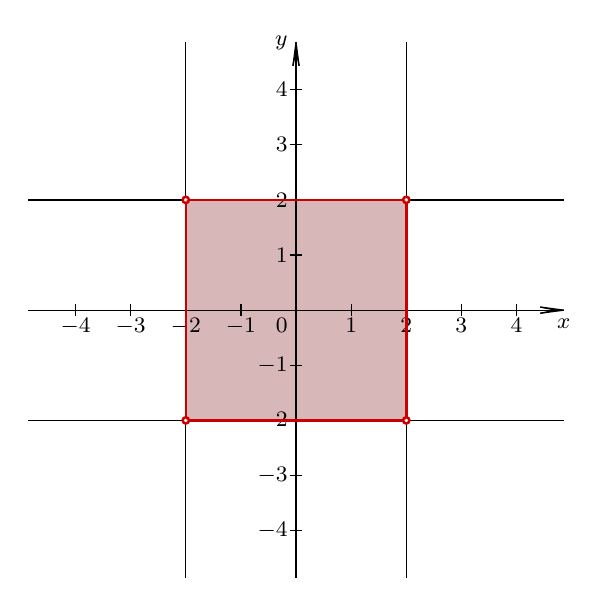
\begin{tikzpicture}
                            % \clip (0,0) rectangle (14.000000,10.000000);
                            {\footnotesize
                                                        
                            % Changing color 215 183 183
                            \definecolor{r215g183b183}{rgb}{0.843137,0.717647,0.717647}%
                            \color{r215g183b183}% 
                            
                            % Filling rectangle left-bottom: X right-top: Y
                            \fill (2.600000,2.600000) -- (5.400000,2.600000) -- (5.400000,5.400000) -- (2.600000,5.400000);%
                            
                            % Changing color 0 0 0
                            \definecolor{r0g0b0}{rgb}{0.000000,0.000000,0.000000}%
                            \color{r0g0b0}% 
                            
                            % Drawing 2D Cartesian system
                            \draw (4.000000,4.000000) node [anchor=north east] { $0$ };%
                            \draw [line width=0.016cm] (4.000000,3.925000) -- (4.000000,4.075000);%
                            \draw (4.700000,4.000000) node [anchor=north] { $1$ };%
                            \draw [line width=0.016cm] (4.700000,3.925000) -- (4.700000,4.075000);%
                            \draw (5.400000,4.000000) node [anchor=north] { $2$ };%
                            \draw [line width=0.016cm] (5.400000,3.925000) -- (5.400000,4.075000);%
                            \draw (6.100000,4.000000) node [anchor=north] { $3$ };%
                            \draw [line width=0.016cm] (6.100000,3.925000) -- (6.100000,4.075000);%
                            \draw (6.800000,4.000000) node [anchor=north] { $4$ };%
                            \draw [line width=0.016cm] (6.800000,3.925000) -- (6.800000,4.075000);%
                            \draw (3.300000,4.000000) node [anchor=north] { $-1$ };%
                            \draw [line width=0.016cm] (3.300000,3.925000) -- (3.300000,4.075000);%
                            \draw (2.600000,4.000000) node [anchor=north] { $-2$ };%
                            \draw [line width=0.016cm] (2.600000,3.925000) -- (2.600000,4.075000);%
                            \draw (1.900000,4.000000) node [anchor=north] { $-3$ };%
                            \draw [line width=0.016cm] (1.900000,3.925000) -- (1.900000,4.075000);%
                            \draw (1.200000,4.000000) node [anchor=north] { $-4$ };%
                            \draw [line width=0.016cm] (1.200000,3.925000) -- (1.200000,4.075000);%
                            \draw (4.000000,4.700000) node [anchor=east] { $1$ };%
                            \draw [line width=0.016cm] (3.925000,4.700000) -- (4.075000,4.700000);%
                            \draw (4.000000,5.400000) node [anchor=east] { $2$ };%
                            \draw [line width=0.016cm] (3.925000,5.400000) -- (4.075000,5.400000);%
                            \draw (4.000000,6.100000) node [anchor=east] { $3$ };%
                            \draw [line width=0.016cm] (3.925000,6.100000) -- (4.075000,6.100000);%
                            \draw (4.000000,6.800000) node [anchor=east] { $4$ };%
                            \draw [line width=0.016cm] (3.925000,6.800000) -- (4.075000,6.800000);%
                            \draw (4.000000,3.300000) node [anchor=east] { $-1$ };%
                            \draw [line width=0.016cm] (3.925000,3.300000) -- (4.075000,3.300000);%
                            \draw (4.000000,2.600000) node [anchor=east] { $-2$ };%
                            \draw [line width=0.016cm] (3.925000,2.600000) -- (4.075000,2.600000);%
                            \draw (4.000000,1.900000) node [anchor=east] { $-3$ };%
                            \draw [line width=0.016cm] (3.925000,1.900000) -- (4.075000,1.900000);%
                            \draw (4.000000,1.200000) node [anchor=east] { $-4$ };%
                            \draw [line width=0.016cm] (3.925000,1.200000) -- (4.075000,1.200000);%
                            \draw (7.400000,4.000000) node [anchor=north] { $x$ };%
                            \draw (4.000000,7.400000) node [anchor=east] { $y$ };%
                            \draw [line width=0.016cm] (0.600000,4.000000) -- (7.400000,4.000000);%
                            \draw [line width=0.016cm] (7.102567,4.039158) -- (7.400000,4.000000);%
                            \draw [line width=0.016cm] (7.102567,4.039158) -- (7.300000,4.000000);%
                            \draw [line width=0.016cm] (7.102567,3.960842) -- (7.400000,4.000000);%
                            \draw [line width=0.016cm] (7.102567,3.960842) -- (7.300000,4.000000);%
                            \draw [line width=0.016cm] (4.000000,0.600000) -- (4.000000,7.400000);%
                            \draw [line width=0.016cm] (3.960842,7.102567) -- (4.000000,7.400000);%
                            \draw [line width=0.016cm] (3.960842,7.102567) -- (4.000000,7.300000);%
                            \draw [line width=0.016cm] (4.039158,7.102567) -- (4.000000,7.400000);%
                            \draw [line width=0.016cm] (4.039158,7.102567) -- (4.000000,7.300000);%
                            
                            % Drawing line A B
                            \draw [line width=0.016cm] (0.600000,2.600000) -- (2.560000,2.600000);%
                            \draw [line width=0.016cm] (2.640000,2.600000) -- (5.360000,2.600000);%
                            \draw [line width=0.016cm] (5.440000,2.600000) -- (7.400000,2.600000);%
                            
                            % Drawing line B C
                            \draw [line width=0.016cm] (5.400000,0.600000) -- (5.400000,2.560000);%
                            \draw [line width=0.016cm] (5.400000,2.640000) -- (5.400000,5.360000);%
                            \draw [line width=0.016cm] (5.400000,5.440000) -- (5.400000,7.400000);%
                            
                            % Drawing line C D
                            \draw [line width=0.016cm] (0.600000,5.400000) -- (2.560000,5.400000);%
                            \draw [line width=0.016cm] (2.640000,5.400000) -- (5.360000,5.400000);%
                            \draw [line width=0.016cm] (5.440000,5.400000) -- (7.400000,5.400000);%
                            
                            % Drawing line A D
                            \draw [line width=0.016cm] (2.600000,0.600000) -- (2.600000,2.560000);%
                            \draw [line width=0.016cm] (2.600000,2.640000) -- (2.600000,5.360000);%
                            \draw [line width=0.016cm] (2.600000,5.440000) -- (2.600000,7.400000);%
                            
                            % Changing color 204 0 0
                            \definecolor{r204g0b0}{rgb}{0.800000,0.000000,0.000000}%
                            \color{r204g0b0}% 
                            
                            % Drawing segment A B
                            \draw [line width=0.032cm] (2.640000,2.600000) -- (5.360000,2.600000);%
                            
                            % Drawing segment B C
                            \draw [line width=0.032cm] (5.400000,2.640000) -- (5.400000,5.360000);%
                            
                            % Drawing segment C D
                            \draw [line width=0.032cm] (5.360000,5.400000) -- (2.640000,5.400000);%
                            
                            % Drawing segment A D
                            \draw [line width=0.032cm] (2.600000,2.640000) -- (2.600000,5.360000);%
                            
                            % Marking point A by circle
                            \draw [line width=0.032cm] (2.600000,2.600000) circle (0.040000);%
                            
                            % Marking point B by circle
                            \draw [line width=0.032cm] (5.400000,2.600000) circle (0.040000);%
                            
                            % Marking point D by circle
                            \draw [line width=0.032cm] (2.600000,5.400000) circle (0.040000);%
                            
                            % Marking point C by circle
                            \draw [line width=0.032cm] (5.400000,5.400000) circle (0.040000);%
                            \color{black}
                            }
                        \end{tikzpicture}
                            
                    \end{figure}

                    \column{0.48\textwidth}
                    \vskip-1.5em
                    \begin{figure}[H]
                        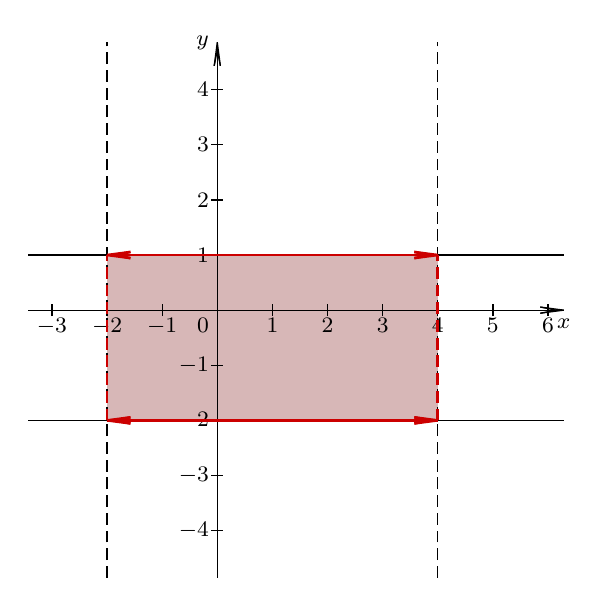
\begin{tikzpicture}
                            % \clip (0,0) rectangle (14.000000,10.000000);
                            {\footnotesize
                                                        
                            % Changing color 215 183 183
                            \definecolor{r215g183b183}{rgb}{0.843137,0.717647,0.717647}%
                            \color{r215g183b183}% 
                            
                            % Filling rectangle left-bottom: X right-top: Y
                            \fill (1.600000,2.600000) -- (5.800000,2.600000) -- (5.800000,4.700000) -- (1.600000,4.700000);%
                            
                            % Changing color 0 0 0
                            \definecolor{r0g0b0}{rgb}{0.000000,0.000000,0.000000}%
                            \color{r0g0b0}% 
                            
                            % Drawing 2D Cartesian system
                            \draw (3.000000,4.000000) node [anchor=north east] { $0$ };%
                            \draw [line width=0.016cm] (3.000000,3.925000) -- (3.000000,4.075000);%
                            \draw (3.700000,4.000000) node [anchor=north] { $1$ };%
                            \draw [line width=0.016cm] (3.700000,3.925000) -- (3.700000,4.075000);%
                            \draw (4.400000,4.000000) node [anchor=north] { $2$ };%
                            \draw [line width=0.016cm] (4.400000,3.925000) -- (4.400000,4.075000);%
                            \draw (5.100000,4.000000) node [anchor=north] { $3$ };%
                            \draw [line width=0.016cm] (5.100000,3.925000) -- (5.100000,4.075000);%
                            \draw (5.800000,4.000000) node [anchor=north] { $4$ };%
                            \draw [line width=0.016cm] (5.800000,3.925000) -- (5.800000,4.075000);%
                            \draw (6.500000,4.000000) node [anchor=north] { $5$ };%
                            \draw [line width=0.016cm] (6.500000,3.925000) -- (6.500000,4.075000);%
                            \draw (7.200000,4.000000) node [anchor=north] { $6$ };%
                            \draw [line width=0.016cm] (7.200000,3.925000) -- (7.200000,4.075000);%
                            \draw (2.300000,4.000000) node [anchor=north] { $-1$ };%
                            \draw [line width=0.016cm] (2.300000,3.925000) -- (2.300000,4.075000);%
                            \draw (1.600000,4.000000) node [anchor=north] { $-2$ };%
                            \draw [line width=0.016cm] (1.600000,3.925000) -- (1.600000,4.075000);%
                            \draw (0.900000,4.000000) node [anchor=north] { $-3$ };%
                            \draw [line width=0.016cm] (0.900000,3.925000) -- (0.900000,4.075000);%
                            \draw (3.000000,4.700000) node [anchor=east] { $1$ };%
                            \draw [line width=0.016cm] (2.925000,4.700000) -- (3.075000,4.700000);%
                            \draw (3.000000,5.400000) node [anchor=east] { $2$ };%
                            \draw [line width=0.016cm] (2.925000,5.400000) -- (3.075000,5.400000);%
                            \draw (3.000000,6.100000) node [anchor=east] { $3$ };%
                            \draw [line width=0.016cm] (2.925000,6.100000) -- (3.075000,6.100000);%
                            \draw (3.000000,6.800000) node [anchor=east] { $4$ };%
                            \draw [line width=0.016cm] (2.925000,6.800000) -- (3.075000,6.800000);%
                            \draw (3.000000,3.300000) node [anchor=east] { $-1$ };%
                            \draw [line width=0.016cm] (2.925000,3.300000) -- (3.075000,3.300000);%
                            \draw (3.000000,2.600000) node [anchor=east] { $-2$ };%
                            \draw [line width=0.016cm] (2.925000,2.600000) -- (3.075000,2.600000);%
                            \draw (3.000000,1.900000) node [anchor=east] { $-3$ };%
                            \draw [line width=0.016cm] (2.925000,1.900000) -- (3.075000,1.900000);%
                            \draw (3.000000,1.200000) node [anchor=east] { $-4$ };%
                            \draw [line width=0.016cm] (2.925000,1.200000) -- (3.075000,1.200000);%
                            \draw (7.400000,4.000000) node [anchor=north] { $x$ };%
                            \draw (3.000000,7.400000) node [anchor=east] { $y$ };%
                            \draw [line width=0.016cm] (0.600000,4.000000) -- (7.400000,4.000000);%
                            \draw [line width=0.016cm] (7.102567,4.039158) -- (7.400000,4.000000);%
                            \draw [line width=0.016cm] (7.102567,4.039158) -- (7.300000,4.000000);%
                            \draw [line width=0.016cm] (7.102567,3.960842) -- (7.400000,4.000000);%
                            \draw [line width=0.016cm] (7.102567,3.960842) -- (7.300000,4.000000);%
                            \draw [line width=0.016cm] (3.000000,0.600000) -- (3.000000,7.400000);%
                            \draw [line width=0.016cm] (2.960842,7.102567) -- (3.000000,7.400000);%
                            \draw [line width=0.016cm] (2.960842,7.102567) -- (3.000000,7.300000);%
                            \draw [line width=0.016cm] (3.039158,7.102567) -- (3.000000,7.400000);%
                            \draw [line width=0.016cm] (3.039158,7.102567) -- (3.000000,7.300000);%
                            
                            % Drawing line A B
                            \draw [line width=0.016cm] (0.600000,2.600000) -- (7.400000,2.600000);%
                            
                            % Drawing line B C
                            \draw [line width=0.016cm] (5.800000,0.600000) -- (5.800000,0.750000);%
                            \draw [line width=0.016cm] (5.800000,0.825000) -- (5.800000,0.975000);%
                            \draw [line width=0.016cm] (5.800000,1.050000) -- (5.800000,1.200000);%
                            \draw [line width=0.016cm] (5.800000,1.275000) -- (5.800000,1.425000);%
                            \draw [line width=0.016cm] (5.800000,1.500000) -- (5.800000,1.650000);%
                            \draw [line width=0.016cm] (5.800000,1.725000) -- (5.800000,1.875000);%
                            \draw [line width=0.016cm] (5.800000,1.950000) -- (5.800000,2.100000);%
                            \draw [line width=0.016cm] (5.800000,2.175000) -- (5.800000,2.325000);%
                            \draw [line width=0.016cm] (5.800000,2.400000) -- (5.800000,2.550000);%
                            \draw [line width=0.016cm] (5.800000,2.625000) -- (5.800000,2.775000);%
                            \draw [line width=0.016cm] (5.800000,2.850000) -- (5.800000,3.000000);%
                            \draw [line width=0.016cm] (5.800000,3.075000) -- (5.800000,3.225000);%
                            \draw [line width=0.016cm] (5.800000,3.300000) -- (5.800000,3.450000);%
                            \draw [line width=0.016cm] (5.800000,3.525000) -- (5.800000,3.675000);%
                            \draw [line width=0.016cm] (5.800000,3.750000) -- (5.800000,3.900000);%
                            \draw [line width=0.016cm] (5.800000,3.975000) -- (5.800000,4.125000);%
                            \draw [line width=0.016cm] (5.800000,4.200000) -- (5.800000,4.350000);%
                            \draw [line width=0.016cm] (5.800000,4.425000) -- (5.800000,4.575000);%
                            \draw [line width=0.016cm] (5.800000,4.650000) -- (5.800000,4.800000);%
                            \draw [line width=0.016cm] (5.800000,4.875000) -- (5.800000,5.025000);%
                            \draw [line width=0.016cm] (5.800000,5.100000) -- (5.800000,5.250000);%
                            \draw [line width=0.016cm] (5.800000,5.325000) -- (5.800000,5.475000);%
                            \draw [line width=0.016cm] (5.800000,5.550000) -- (5.800000,5.700000);%
                            \draw [line width=0.016cm] (5.800000,5.775000) -- (5.800000,5.925000);%
                            \draw [line width=0.016cm] (5.800000,6.000000) -- (5.800000,6.150000);%
                            \draw [line width=0.016cm] (5.800000,6.225000) -- (5.800000,6.375000);%
                            \draw [line width=0.016cm] (5.800000,6.450000) -- (5.800000,6.600000);%
                            \draw [line width=0.016cm] (5.800000,6.675000) -- (5.800000,6.825000);%
                            \draw [line width=0.016cm] (5.800000,6.900000) -- (5.800000,7.050000);%
                            \draw [line width=0.016cm] (5.800000,7.125000) -- (5.800000,7.275000);%
                            \draw [line width=0.016cm] (5.800000,7.350000) -- (5.800000,7.400000);%
                            
                            % Drawing line C D
                            \draw [line width=0.016cm] (0.600000,4.700000) -- (7.400000,4.700000);%
                            
                            % Drawing line A D
                            \draw [line width=0.016cm] (1.600000,0.600000) -- (1.600000,0.750000);%
                            \draw [line width=0.016cm] (1.600000,0.825000) -- (1.600000,0.975000);%
                            \draw [line width=0.016cm] (1.600000,1.050000) -- (1.600000,1.200000);%
                            \draw [line width=0.016cm] (1.600000,1.275000) -- (1.600000,1.425000);%
                            \draw [line width=0.016cm] (1.600000,1.500000) -- (1.600000,1.650000);%
                            \draw [line width=0.016cm] (1.600000,1.725000) -- (1.600000,1.875000);%
                            \draw [line width=0.016cm] (1.600000,1.950000) -- (1.600000,2.100000);%
                            \draw [line width=0.016cm] (1.600000,2.175000) -- (1.600000,2.325000);%
                            \draw [line width=0.016cm] (1.600000,2.400000) -- (1.600000,2.550000);%
                            \draw [line width=0.016cm] (1.600000,2.625000) -- (1.600000,2.775000);%
                            \draw [line width=0.016cm] (1.600000,2.850000) -- (1.600000,3.000000);%
                            \draw [line width=0.016cm] (1.600000,3.075000) -- (1.600000,3.225000);%
                            \draw [line width=0.016cm] (1.600000,3.300000) -- (1.600000,3.450000);%
                            \draw [line width=0.016cm] (1.600000,3.525000) -- (1.600000,3.675000);%
                            \draw [line width=0.016cm] (1.600000,3.750000) -- (1.600000,3.900000);%
                            \draw [line width=0.016cm] (1.600000,3.975000) -- (1.600000,4.125000);%
                            \draw [line width=0.016cm] (1.600000,4.200000) -- (1.600000,4.350000);%
                            \draw [line width=0.016cm] (1.600000,4.425000) -- (1.600000,4.575000);%
                            \draw [line width=0.016cm] (1.600000,4.650000) -- (1.600000,4.800000);%
                            \draw [line width=0.016cm] (1.600000,4.875000) -- (1.600000,5.025000);%
                            \draw [line width=0.016cm] (1.600000,5.100000) -- (1.600000,5.250000);%
                            \draw [line width=0.016cm] (1.600000,5.325000) -- (1.600000,5.475000);%
                            \draw [line width=0.016cm] (1.600000,5.550000) -- (1.600000,5.700000);%
                            \draw [line width=0.016cm] (1.600000,5.775000) -- (1.600000,5.925000);%
                            \draw [line width=0.016cm] (1.600000,6.000000) -- (1.600000,6.150000);%
                            \draw [line width=0.016cm] (1.600000,6.225000) -- (1.600000,6.375000);%
                            \draw [line width=0.016cm] (1.600000,6.450000) -- (1.600000,6.600000);%
                            \draw [line width=0.016cm] (1.600000,6.675000) -- (1.600000,6.825000);%
                            \draw [line width=0.016cm] (1.600000,6.900000) -- (1.600000,7.050000);%
                            \draw [line width=0.016cm] (1.600000,7.125000) -- (1.600000,7.275000);%
                            \draw [line width=0.016cm] (1.600000,7.350000) -- (1.600000,7.400000);%
                            
                            % Changing color 204 0 0
                            \definecolor{r204g0b0}{rgb}{0.800000,0.000000,0.000000}%
                            \color{r204g0b0}% 
                            
                            % Drawing segment A B
                            \draw [line width=0.032cm] (1.600000,2.600000) -- (5.800000,2.600000);%
                            
                            % Drawing segment B C
                            \draw [line width=0.032cm] (5.800000,2.600000) -- (5.800000,2.750000);%
                            \draw [line width=0.032cm] (5.800000,2.825000) -- (5.800000,2.975000);%
                            \draw [line width=0.032cm] (5.800000,3.050000) -- (5.800000,3.200000);%
                            \draw [line width=0.032cm] (5.800000,3.275000) -- (5.800000,3.425000);%
                            \draw [line width=0.032cm] (5.800000,3.500000) -- (5.800000,3.650000);%
                            \draw [line width=0.032cm] (5.800000,3.725000) -- (5.800000,3.875000);%
                            \draw [line width=0.032cm] (5.800000,3.950000) -- (5.800000,4.100000);%
                            \draw [line width=0.032cm] (5.800000,4.175000) -- (5.800000,4.325000);%
                            \draw [line width=0.032cm] (5.800000,4.400000) -- (5.800000,4.550000);%
                            \draw [line width=0.032cm] (5.800000,4.625000) -- (5.800000,4.700000);%
                            
                            % Drawing segment C D
                            \draw [line width=0.032cm] (5.800000,4.700000) -- (1.600000,4.700000);%
                            
                            % Drawing segment A D
                            \draw [line width=0.032cm] (1.600000,2.600000) -- (1.600000,2.750000);%
                            \draw [line width=0.032cm] (1.600000,2.825000) -- (1.600000,2.975000);%
                            \draw [line width=0.032cm] (1.600000,3.050000) -- (1.600000,3.200000);%
                            \draw [line width=0.032cm] (1.600000,3.275000) -- (1.600000,3.425000);%
                            \draw [line width=0.032cm] (1.600000,3.500000) -- (1.600000,3.650000);%
                            \draw [line width=0.032cm] (1.600000,3.725000) -- (1.600000,3.875000);%
                            \draw [line width=0.032cm] (1.600000,3.950000) -- (1.600000,4.100000);%
                            \draw [line width=0.032cm] (1.600000,4.175000) -- (1.600000,4.325000);%
                            \draw [line width=0.032cm] (1.600000,4.400000) -- (1.600000,4.550000);%
                            \draw [line width=0.032cm] (1.600000,4.625000) -- (1.600000,4.700000);%
                            
                            % Drawing arrow A B 1.00
                            \draw [line width=0.032cm] (5.502567,2.639158) -- (5.800000,2.600000);%
                            \draw [line width=0.032cm] (5.502567,2.639158) -- (5.700856,2.600000);%
                            \draw [line width=0.032cm] (5.502567,2.560842) -- (5.800000,2.600000);%
                            \draw [line width=0.032cm] (5.502567,2.560842) -- (5.700856,2.600000);%
                            
                            % Drawing arrow B A 1.00
                            \draw [line width=0.032cm] (1.897433,2.560842) -- (1.600000,2.600000);%
                            \draw [line width=0.032cm] (1.897433,2.560842) -- (1.699144,2.600000);%
                            \draw [line width=0.032cm] (1.897433,2.639158) -- (1.600000,2.600000);%
                            \draw [line width=0.032cm] (1.897433,2.639158) -- (1.699144,2.600000);%
                            
                            % Drawing arrow C D 1.00
                            \draw [line width=0.032cm] (1.897433,4.660842) -- (1.600000,4.700000);%
                            \draw [line width=0.032cm] (1.897433,4.660842) -- (1.699144,4.700000);%
                            \draw [line width=0.032cm] (1.897433,4.739158) -- (1.600000,4.700000);%
                            \draw [line width=0.032cm] (1.897433,4.739158) -- (1.699144,4.700000);%
                            
                            % Drawing arrow D C 1.00
                            \draw [line width=0.032cm] (5.502567,4.739158) -- (5.800000,4.700000);%
                            \draw [line width=0.032cm] (5.502567,4.739158) -- (5.700856,4.700000);%
                            \draw [line width=0.032cm] (5.502567,4.660842) -- (5.800000,4.700000);%
                            \draw [line width=0.032cm] (5.502567,4.660842) -- (5.700856,4.700000);%
                            \color{black}
                            }
                        \end{tikzpicture}
                            
                    \end{figure}

                \end{columns}
            \end{exampleblock}}

        \end{frame}


        
        \begin{frame}

            \only<2->{\begin{exampleblock}{Naloga}
                V koordinatnem sistemu narišite točke $A(-2,3)$, $B(0,4)$, $C(0.5,-1)$ in $D(-3,-1)$.
                \begin{itemize}
                    \item Točke $A$, $B$, $C$ in $D$ prezrcalite čez abscisno os in zapišite koordinate točk $A_1$, $B_1$, $C_1$ in $D_1$.
                    \item Točke $A$, $B$, $C$ in $D$ prezrcalite čez ordinatno os in zapišite koordinate točk $A_2$, $B_2$, $C_2$ in $D_2$.
                    \item Točke $A$, $B$, $C$ in $D$ prezrcalite čez koordinatno izhodišče in zapišite koordinate točk $A_3$, $B_3$, $C_3$ in $D_3$.

                \end{itemize}
            \end{exampleblock}}

        \end{frame}


        \begin{frame}

            \only<2->{\begin{exampleblock}{Naloga}
                V koordinatni sistem narišite točke $(x,y)$ kartezičnega produkta.
                \begin{itemize}
                    \item $[-2,3)\times[-5,-1]$
                    \item $(-1,2)\times[2,3]$
                    \item $\left\{2\right\}\times(3,5]$
                    \item $[-2,3]\times\left\{3,4\right\}$
                    \item $\left\{1,2,3\right\}\times\left\{-1,1\right\}$
                    \item $(0,\infty)\times(1,2)$
                    \item $[-1,3]\times(-\infty,3]$
                    \item $(-1,3]\times\left\{2\right\}$
                \end{itemize}
            \end{exampleblock}}

        \end{frame}






    \subsection{Razdalja med točkama in razpolovišče daljice}

        \begin{frame}
            \frametitle{Razdalja med točkama}

            \vskip-1.7em
            \begin{columns}
                \column{0.54\textwidth}
                \only<2->{\begin{alertblock}{Razdalja med točkama}
                    \only<3->{Razdalja $d(A,B)$ med dvema točkama $A(x_a,y_a)$ in $B(x_b,y_b)$ v ravnini je}
                    \vskip-0.5em
                    \only<4->{$$ d(A,B)=\sqrt{(x_b-x_a)^2+(y_b-y_a)^2}. $$}
                \end{alertblock}}

                \only<5->{\begin{block}{Lastnosti razdalje}
                    \begin{itemize}
                        \item<6-> $d(A,B)\geq 0$
                        \item<7-> $d(A,B)=0\Leftrightarrow A=B$
                        \item<8-> $d(A,B)=d(B,A)$
                        \item<9-> $d(A,C)\leq d(A,B)+d(B,C)$
                    \end{itemize}
                \end{block}}

                \column{0.43\textwidth}

                \only<3->{\begin{block}{}
                    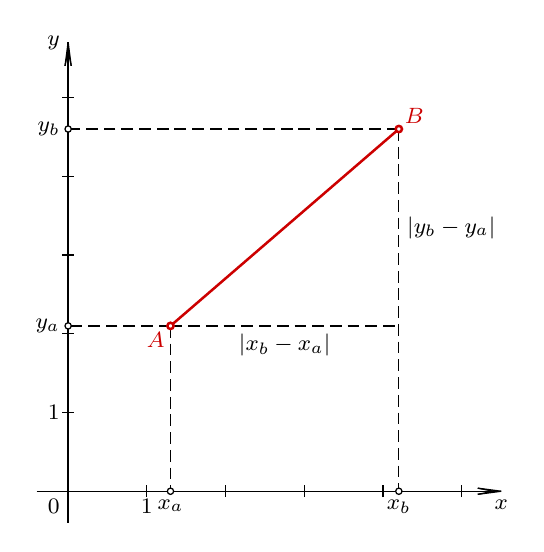
\begin{tikzpicture}
                        % \clip (0,0) rectangle (14.000000,10.000000);
                        {\footnotesize
                        
                        % Drawing 2D Cartesian system
                        \draw (2.000000,2.000000) node [anchor=north east] { $0$ };%
                        \draw [line width=0.016cm] (2.000000,1.925000) -- (2.000000,2.075000);%
                        \draw (3.000000,2.000000) node [anchor=north] { $1$ };%
                        \draw [line width=0.016cm] (3.000000,1.925000) -- (3.000000,2.075000);%
                        % \draw (4.000000,2.000000) node [anchor=north] { $2$ };%
                        \draw [line width=0.016cm] (4.000000,1.925000) -- (4.000000,2.075000);%
                        % \draw (5.000000,2.000000) node [anchor=north] { $3$ };%
                        \draw [line width=0.016cm] (5.000000,1.925000) -- (5.000000,2.075000);%
                        % \draw (6.000000,2.000000) node [anchor=north] { $4$ };%
                        \draw [line width=0.016cm] (6.000000,1.925000) -- (6.000000,2.075000);%
                        % \draw (7.000000,2.000000) node [anchor=north] { $5$ };%
                        \draw [line width=0.016cm] (7.000000,1.925000) -- (7.000000,2.075000);%
                        \draw (2.000000,3.000000) node [anchor=east] { $1$ };%
                        \draw [line width=0.016cm] (1.925000,3.000000) -- (2.075000,3.000000);%
                        % \draw (2.000000,4.000000) node [anchor=east] { $2$ };%
                        \draw [line width=0.016cm] (1.925000,4.000000) -- (2.075000,4.000000);%
                        % \draw (2.000000,5.000000) node [anchor=east] { $3$ };%
                        \draw [line width=0.016cm] (1.925000,5.000000) -- (2.075000,5.000000);%
                        % \draw (2.000000,6.000000) node [anchor=east] { $4$ };%
                        \draw [line width=0.016cm] (1.925000,6.000000) -- (2.075000,6.000000);%
                        % \draw (2.000000,7.000000) node [anchor=east] { $5$ };%
                        \draw [line width=0.016cm] (1.925000,7.000000) -- (2.075000,7.000000);%
                        \draw (7.500000,2.000000) node [anchor=north] { $x$ };%
                        \draw (2.000000,7.700000) node [anchor=east] { $y$ };%
                        \draw [line width=0.016cm] (1.600000,2.000000) -- (3.260000,2.000000);%
                        \draw [line width=0.016cm] (3.340000,2.000000) -- (6.160000,2.000000);%
                        \draw [line width=0.016cm] (6.240000,2.000000) -- (7.500000,2.000000);%
                        \draw [line width=0.016cm] (7.202567,2.039158) -- (7.500000,2.000000);%
                        \draw [line width=0.016cm] (7.202567,2.039158) -- (7.400000,2.000000);%
                        \draw [line width=0.016cm] (7.202567,1.960842) -- (7.500000,2.000000);%
                        \draw [line width=0.016cm] (7.202567,1.960842) -- (7.400000,2.000000);%
                        \draw [line width=0.016cm] (2.000000,1.600000) -- (2.000000,4.060000);%
                        \draw [line width=0.016cm] (2.000000,4.140000) -- (2.000000,6.560000);%
                        \draw [line width=0.016cm] (2.000000,6.640000) -- (2.000000,7.700000);%
                        \draw [line width=0.016cm] (1.960842,7.402567) -- (2.000000,7.700000);%
                        \draw [line width=0.016cm] (1.960842,7.402567) -- (2.000000,7.600000);%
                        \draw [line width=0.016cm] (2.039158,7.402567) -- (2.000000,7.700000);%
                        \draw [line width=0.016cm] (2.039158,7.402567) -- (2.000000,7.600000);%
                        
                        % Drawing segment A x_a
                        \draw [line width=0.016cm] (3.300000,4.060000) -- (3.300000,3.950000);%
                        \draw [line width=0.016cm] (3.300000,3.875000) -- (3.300000,3.725000);%
                        \draw [line width=0.016cm] (3.300000,3.650000) -- (3.300000,3.500000);%
                        \draw [line width=0.016cm] (3.300000,3.425000) -- (3.300000,3.275000);%
                        \draw [line width=0.016cm] (3.300000,3.200000) -- (3.300000,3.050000);%
                        \draw [line width=0.016cm] (3.300000,2.975000) -- (3.300000,2.825000);%
                        \draw [line width=0.016cm] (3.300000,2.750000) -- (3.300000,2.600000);%
                        \draw [line width=0.016cm] (3.300000,2.525000) -- (3.300000,2.375000);%
                        \draw [line width=0.016cm] (3.300000,2.300000) -- (3.300000,2.150000);%
                        \draw [line width=0.016cm] (3.300000,2.075000) -- (3.300000,2.040000);%
                        
                        % Drawing segment A y_a
                        \draw [line width=0.016cm] (3.260000,4.100000) -- (3.150000,4.100000);%
                        \draw [line width=0.016cm] (3.075000,4.100000) -- (2.925000,4.100000);%
                        \draw [line width=0.016cm] (2.850000,4.100000) -- (2.700000,4.100000);%
                        \draw [line width=0.016cm] (2.625000,4.100000) -- (2.475000,4.100000);%
                        \draw [line width=0.016cm] (2.400000,4.100000) -- (2.250000,4.100000);%
                        \draw [line width=0.016cm] (2.175000,4.100000) -- (2.040000,4.100000);%
                        
                        % Drawing segment B x_b
                        \draw [line width=0.016cm] (6.200000,6.560000) -- (6.200000,6.450000);%
                        \draw [line width=0.016cm] (6.200000,6.375000) -- (6.200000,6.225000);%
                        \draw [line width=0.016cm] (6.200000,6.150000) -- (6.200000,6.000000);%
                        \draw [line width=0.016cm] (6.200000,5.925000) -- (6.200000,5.775000);%
                        \draw [line width=0.016cm] (6.200000,5.700000) -- (6.200000,5.550000);%
                        \draw [line width=0.016cm] (6.200000,5.475000) -- (6.200000,5.325000);%
                        \draw [line width=0.016cm] (6.200000,5.250000) -- (6.200000,5.100000);%
                        \draw [line width=0.016cm] (6.200000,5.025000) -- (6.200000,4.875000);%
                        \draw [line width=0.016cm] (6.200000,4.800000) -- (6.200000,4.650000);%
                        \draw [line width=0.016cm] (6.200000,4.575000) -- (6.200000,4.425000);%
                        \draw [line width=0.016cm] (6.200000,4.350000) -- (6.200000,4.200000);%
                        \draw [line width=0.016cm] (6.200000,4.125000) -- (6.200000,3.975000);%
                        \draw [line width=0.016cm] (6.200000,3.900000) -- (6.200000,3.750000);%
                        \draw [line width=0.016cm] (6.200000,3.675000) -- (6.200000,3.525000);%
                        \draw [line width=0.016cm] (6.200000,3.450000) -- (6.200000,3.300000);%
                        \draw [line width=0.016cm] (6.200000,3.225000) -- (6.200000,3.075000);%
                        \draw [line width=0.016cm] (6.200000,3.000000) -- (6.200000,2.850000);%
                        \draw [line width=0.016cm] (6.200000,2.775000) -- (6.200000,2.625000);%
                        \draw [line width=0.016cm] (6.200000,2.550000) -- (6.200000,2.400000);%
                        \draw [line width=0.016cm] (6.200000,2.325000) -- (6.200000,2.175000);%
                        \draw [line width=0.016cm] (6.200000,2.100000) -- (6.200000,2.040000);%
                        
                        % Drawing segment B y_b
                        \draw [line width=0.016cm] (6.160000,6.600000) -- (6.050000,6.600000);%
                        \draw [line width=0.016cm] (5.975000,6.600000) -- (5.825000,6.600000);%
                        \draw [line width=0.016cm] (5.750000,6.600000) -- (5.600000,6.600000);%
                        \draw [line width=0.016cm] (5.525000,6.600000) -- (5.375000,6.600000);%
                        \draw [line width=0.016cm] (5.300000,6.600000) -- (5.150000,6.600000);%
                        \draw [line width=0.016cm] (5.075000,6.600000) -- (4.925000,6.600000);%
                        \draw [line width=0.016cm] (4.850000,6.600000) -- (4.700000,6.600000);%
                        \draw [line width=0.016cm] (4.625000,6.600000) -- (4.475000,6.600000);%
                        \draw [line width=0.016cm] (4.400000,6.600000) -- (4.250000,6.600000);%
                        \draw [line width=0.016cm] (4.175000,6.600000) -- (4.025000,6.600000);%
                        \draw [line width=0.016cm] (3.950000,6.600000) -- (3.800000,6.600000);%
                        \draw [line width=0.016cm] (3.725000,6.600000) -- (3.575000,6.600000);%
                        \draw [line width=0.016cm] (3.500000,6.600000) -- (3.350000,6.600000);%
                        \draw [line width=0.016cm] (3.275000,6.600000) -- (3.125000,6.600000);%
                        \draw [line width=0.016cm] (3.050000,6.600000) -- (2.900000,6.600000);%
                        \draw [line width=0.016cm] (2.825000,6.600000) -- (2.675000,6.600000);%
                        \draw [line width=0.016cm] (2.600000,6.600000) -- (2.450000,6.600000);%
                        \draw [line width=0.016cm] (2.375000,6.600000) -- (2.225000,6.600000);%
                        \draw [line width=0.016cm] (2.150000,6.600000) -- (2.040000,6.600000);%
                        
                        \only<4->{% Drawing segment A xy
                        \draw [line width=0.016cm] (3.340000,4.100000) -- (3.450000,4.100000);%
                        \draw [line width=0.016cm] (3.525000,4.100000) -- (3.675000,4.100000);%
                        \draw [line width=0.016cm] (3.750000,4.100000) -- (3.900000,4.100000);%
                        \draw [line width=0.016cm] (3.975000,4.100000) -- (4.125000,4.100000);%
                        \draw [line width=0.016cm] (4.200000,4.100000) -- (4.350000,4.100000);%
                        \draw [line width=0.016cm] (4.425000,4.100000) -- (4.575000,4.100000);%
                        \draw [line width=0.016cm] (4.650000,4.100000) -- (4.800000,4.100000);%
                        \draw [line width=0.016cm] (4.875000,4.100000) -- (5.025000,4.100000);%
                        \draw [line width=0.016cm] (5.100000,4.100000) -- (5.250000,4.100000);%
                        \draw [line width=0.016cm] (5.325000,4.100000) -- (5.475000,4.100000);%
                        \draw [line width=0.016cm] (5.550000,4.100000) -- (5.700000,4.100000);%
                        \draw [line width=0.016cm] (5.775000,4.100000) -- (5.925000,4.100000);%
                        \draw [line width=0.016cm] (6.000000,4.100000) -- (6.150000,4.100000);%
                        }
                        % Marking point x_a by circle
                        \draw [line width=0.016cm] (3.300000,2.000000) circle (0.040000);%
                        \draw (3.300000,2.000000) node [anchor=north] { $x_a$ };%
                        
                        % Marking point x_b by circle
                        \draw [line width=0.016cm] (6.200000,2.000000) circle (0.040000);%
                        \draw (6.200000,2.000000) node [anchor=north] { $x_b$ };%
                        
                        % Marking point y_a by circle
                        \draw [line width=0.016cm] (2.000000,4.100000) circle (0.040000);%
                        \draw (2.000000,4.100000) node [anchor=east] { $y_a$ };%
                        
                        % Marking point y_b by circle
                        \draw [line width=0.016cm] (2.000000,6.600000) circle (0.040000);%
                        \draw (2.000000,6.600000) node [anchor=east] { $y_b$ };%
                        \only<4->{
                        % Marking point {|x_b-x_a|}
                        \draw (4.750000,4.100000) node [anchor=north] { ${|x_b-x_a|}$ };%
                        
                        % Marking point {|y_b-y_a|}
                        \draw (6.200000,5.350000) node [anchor=west] { ${|y_b-y_a|}$ };%
                        }
                        % Changing color 204 0 0
                        \definecolor{r204g0b0}{rgb}{0.800000,0.000000,0.000000}%
                        \color{r204g0b0}% 
                        
                        % Drawing segment A B
                        \draw [line width=0.032cm] (3.330296,4.126118) -- (6.169704,6.573882);%
                        
                        % Marking point A by circle
                        \draw [line width=0.032cm] (3.300000,4.100000) circle (0.040000);%
                        \draw (3.330000,4.130000) node [anchor=north east] { $A$ };%
                        
                        % Marking point B by circle
                        \draw [line width=0.032cm] (6.200000,6.600000) circle (0.040000);%
                        \draw (6.170000,6.570000) node [anchor=south west] { $B$ };%
                        \color{black}
                        }
                        \end{tikzpicture}
                        
                \end{block}}
            \end{columns}

        \end{frame}


        \begin{frame}
            \frametitle{Razpolovišče daljice}
            
            \vskip-1.7em
            \begin{columns}
                \column{0.52\textwidth}

                \only<2->{\begin{alertblock}{Razpolovišče daljice}
                    \only<3->{Razpolovišče $S$ daljice $AB$ s krajiščema $A(x_a,y_a)$ in $B(x_b,y_b)$ v ravnini je}
                    \only<4->{$$ S\left(\dfrac{x_a+x_b}{2},\dfrac{y_a+y_b}{2}\right). $$}
                \end{alertblock}}
                \column{0.43\textwidth}

                \only<3->{\begin{block}{}
                    \begin{tikzpicture}
                        % \clip (0,0) rectangle (14.000000,10.000000);
                        {\footnotesize
                        
                        % Drawing 2D Cartesian system
                        \draw (2.000000,2.000000) node [anchor=north east] { $0$ };%
                        \draw [line width=0.016cm] (2.000000,1.925000) -- (2.000000,2.075000);%
                        \draw (3.000000,2.000000) node [anchor=north] { $1$ };%
                        \draw [line width=0.016cm] (3.000000,1.925000) -- (3.000000,2.075000);%
                        % \draw (4.000000,2.000000) node [anchor=north] { $2$ };%
                        \draw [line width=0.016cm] (4.000000,1.925000) -- (4.000000,2.075000);%
                        % \draw (5.000000,2.000000) node [anchor=north] { $3$ };%
                        \draw [line width=0.016cm] (5.000000,1.925000) -- (5.000000,2.075000);%
                        % \draw (6.000000,2.000000) node [anchor=north] { $4$ };%
                        \draw [line width=0.016cm] (6.000000,1.925000) -- (6.000000,2.075000);%
                        % \draw (7.000000,2.000000) node [anchor=north] { $5$ };%
                        \draw [line width=0.016cm] (7.000000,1.925000) -- (7.000000,2.075000);%
                        \draw (2.000000,3.000000) node [anchor=east] { $1$ };%
                        \draw [line width=0.016cm] (1.925000,3.000000) -- (2.075000,3.000000);%
                        % \draw (2.000000,4.000000) node [anchor=east] { $2$ };%
                        \draw [line width=0.016cm] (1.925000,4.000000) -- (2.075000,4.000000);%
                        % \draw (2.000000,5.000000) node [anchor=east] { $3$ };%
                        \draw [line width=0.016cm] (1.925000,5.000000) -- (2.075000,5.000000);%
                        % \draw (2.000000,6.000000) node [anchor=east] { $4$ };%
                        \draw [line width=0.016cm] (1.925000,6.000000) -- (2.075000,6.000000);%
                        % \draw (2.000000,7.000000) node [anchor=east] { $5$ };%
                        \draw [line width=0.016cm] (1.925000,7.000000) -- (2.075000,7.000000);%
                        \draw (7.500000,2.000000) node [anchor=north] { $x$ };%
                        \draw (2.000000,7.400000) node [anchor=east] { $y$ };%
                        \draw [line width=0.016cm] (1.300000,2.000000) -- (3.260000,2.000000);%
                        \draw [line width=0.016cm] (3.340000,2.000000) -- (4.710000,2.000000);%
                        \draw [line width=0.016cm] (4.790000,2.000000) -- (6.160000,2.000000);%
                        \draw [line width=0.016cm] (6.240000,2.000000) -- (7.500000,2.000000);%
                        \draw [line width=0.016cm] (7.202567,2.039158) -- (7.500000,2.000000);%
                        \draw [line width=0.016cm] (7.202567,2.039158) -- (7.400000,2.000000);%
                        \draw [line width=0.016cm] (7.202567,1.960842) -- (7.500000,2.000000);%
                        \draw [line width=0.016cm] (7.202567,1.960842) -- (7.400000,2.000000);%
                        \draw [line width=0.016cm] (2.000000,1.300000) -- (2.000000,4.060000);%
                        \draw [line width=0.016cm] (2.000000,4.140000) -- (2.000000,5.310000);%
                        \draw [line width=0.016cm] (2.000000,5.390000) -- (2.000000,6.560000);%
                        \draw [line width=0.016cm] (2.000000,6.640000) -- (2.000000,7.400000);%
                        \draw [line width=0.016cm] (1.960842,7.102567) -- (2.000000,7.400000);%
                        \draw [line width=0.016cm] (1.960842,7.102567) -- (2.000000,7.300000);%
                        \draw [line width=0.016cm] (2.039158,7.102567) -- (2.000000,7.400000);%
                        \draw [line width=0.016cm] (2.039158,7.102567) -- (2.000000,7.300000);%
                        
                        % Drawing segment A x_a
                        \draw [line width=0.016cm] (3.300000,4.060000) -- (3.300000,3.950000);%
                        \draw [line width=0.016cm] (3.300000,3.875000) -- (3.300000,3.725000);%
                        \draw [line width=0.016cm] (3.300000,3.650000) -- (3.300000,3.500000);%
                        \draw [line width=0.016cm] (3.300000,3.425000) -- (3.300000,3.275000);%
                        \draw [line width=0.016cm] (3.300000,3.200000) -- (3.300000,3.050000);%
                        \draw [line width=0.016cm] (3.300000,2.975000) -- (3.300000,2.825000);%
                        \draw [line width=0.016cm] (3.300000,2.750000) -- (3.300000,2.600000);%
                        \draw [line width=0.016cm] (3.300000,2.525000) -- (3.300000,2.375000);%
                        \draw [line width=0.016cm] (3.300000,2.300000) -- (3.300000,2.150000);%
                        \draw [line width=0.016cm] (3.300000,2.075000) -- (3.300000,2.040000);%
                        
                        % Drawing segment A y_a
                        \draw [line width=0.016cm] (3.260000,4.100000) -- (3.150000,4.100000);%
                        \draw [line width=0.016cm] (3.075000,4.100000) -- (2.925000,4.100000);%
                        \draw [line width=0.016cm] (2.850000,4.100000) -- (2.700000,4.100000);%
                        \draw [line width=0.016cm] (2.625000,4.100000) -- (2.475000,4.100000);%
                        \draw [line width=0.016cm] (2.400000,4.100000) -- (2.250000,4.100000);%
                        \draw [line width=0.016cm] (2.175000,4.100000) -- (2.040000,4.100000);%
                        
                        % Drawing segment B x_b
                        \draw [line width=0.016cm] (6.200000,6.560000) -- (6.200000,6.450000);%
                        \draw [line width=0.016cm] (6.200000,6.375000) -- (6.200000,6.225000);%
                        \draw [line width=0.016cm] (6.200000,6.150000) -- (6.200000,6.000000);%
                        \draw [line width=0.016cm] (6.200000,5.925000) -- (6.200000,5.775000);%
                        \draw [line width=0.016cm] (6.200000,5.700000) -- (6.200000,5.550000);%
                        \draw [line width=0.016cm] (6.200000,5.475000) -- (6.200000,5.325000);%
                        \draw [line width=0.016cm] (6.200000,5.250000) -- (6.200000,5.100000);%
                        \draw [line width=0.016cm] (6.200000,5.025000) -- (6.200000,4.875000);%
                        \draw [line width=0.016cm] (6.200000,4.800000) -- (6.200000,4.650000);%
                        \draw [line width=0.016cm] (6.200000,4.575000) -- (6.200000,4.425000);%
                        \draw [line width=0.016cm] (6.200000,4.350000) -- (6.200000,4.200000);%
                        \draw [line width=0.016cm] (6.200000,4.125000) -- (6.200000,3.975000);%
                        \draw [line width=0.016cm] (6.200000,3.900000) -- (6.200000,3.750000);%
                        \draw [line width=0.016cm] (6.200000,3.675000) -- (6.200000,3.525000);%
                        \draw [line width=0.016cm] (6.200000,3.450000) -- (6.200000,3.300000);%
                        \draw [line width=0.016cm] (6.200000,3.225000) -- (6.200000,3.075000);%
                        \draw [line width=0.016cm] (6.200000,3.000000) -- (6.200000,2.850000);%
                        \draw [line width=0.016cm] (6.200000,2.775000) -- (6.200000,2.625000);%
                        \draw [line width=0.016cm] (6.200000,2.550000) -- (6.200000,2.400000);%
                        \draw [line width=0.016cm] (6.200000,2.325000) -- (6.200000,2.175000);%
                        \draw [line width=0.016cm] (6.200000,2.100000) -- (6.200000,2.040000);%
                        
                        % Drawing segment B y_b
                        \draw [line width=0.016cm] (6.160000,6.600000) -- (6.050000,6.600000);%
                        \draw [line width=0.016cm] (5.975000,6.600000) -- (5.825000,6.600000);%
                        \draw [line width=0.016cm] (5.750000,6.600000) -- (5.600000,6.600000);%
                        \draw [line width=0.016cm] (5.525000,6.600000) -- (5.375000,6.600000);%
                        \draw [line width=0.016cm] (5.300000,6.600000) -- (5.150000,6.600000);%
                        \draw [line width=0.016cm] (5.075000,6.600000) -- (4.925000,6.600000);%
                        \draw [line width=0.016cm] (4.850000,6.600000) -- (4.700000,6.600000);%
                        \draw [line width=0.016cm] (4.625000,6.600000) -- (4.475000,6.600000);%
                        \draw [line width=0.016cm] (4.400000,6.600000) -- (4.250000,6.600000);%
                        \draw [line width=0.016cm] (4.175000,6.600000) -- (4.025000,6.600000);%
                        \draw [line width=0.016cm] (3.950000,6.600000) -- (3.800000,6.600000);%
                        \draw [line width=0.016cm] (3.725000,6.600000) -- (3.575000,6.600000);%
                        \draw [line width=0.016cm] (3.500000,6.600000) -- (3.350000,6.600000);%
                        \draw [line width=0.016cm] (3.275000,6.600000) -- (3.125000,6.600000);%
                        \draw [line width=0.016cm] (3.050000,6.600000) -- (2.900000,6.600000);%
                        \draw [line width=0.016cm] (2.825000,6.600000) -- (2.675000,6.600000);%
                        \draw [line width=0.016cm] (2.600000,6.600000) -- (2.450000,6.600000);%
                        \draw [line width=0.016cm] (2.375000,6.600000) -- (2.225000,6.600000);%
                        \draw [line width=0.016cm] (2.150000,6.600000) -- (2.040000,6.600000);%
                        \only<4->{
                        % Drawing segment S x_s
                        \draw [line width=0.016cm] (4.750000,5.310000) -- (4.750000,5.200000);%
                        \draw [line width=0.016cm] (4.750000,5.125000) -- (4.750000,4.975000);%
                        \draw [line width=0.016cm] (4.750000,4.900000) -- (4.750000,4.750000);%
                        \draw [line width=0.016cm] (4.750000,4.675000) -- (4.750000,4.525000);%
                        \draw [line width=0.016cm] (4.750000,4.450000) -- (4.750000,4.300000);%
                        \draw [line width=0.016cm] (4.750000,4.225000) -- (4.750000,4.075000);%
                        \draw [line width=0.016cm] (4.750000,4.000000) -- (4.750000,3.850000);%
                        \draw [line width=0.016cm] (4.750000,3.775000) -- (4.750000,3.625000);%
                        \draw [line width=0.016cm] (4.750000,3.550000) -- (4.750000,3.400000);%
                        \draw [line width=0.016cm] (4.750000,3.325000) -- (4.750000,3.175000);%
                        \draw [line width=0.016cm] (4.750000,3.100000) -- (4.750000,2.950000);%
                        \draw [line width=0.016cm] (4.750000,2.875000) -- (4.750000,2.725000);%
                        \draw [line width=0.016cm] (4.750000,2.650000) -- (4.750000,2.500000);%
                        \draw [line width=0.016cm] (4.750000,2.425000) -- (4.750000,2.275000);%
                        \draw [line width=0.016cm] (4.750000,2.200000) -- (4.750000,2.050000);%
                        
                        % Drawing segment S y_s
                        \draw [line width=0.016cm] (4.710000,5.350000) -- (4.600000,5.350000);%
                        \draw [line width=0.016cm] (4.525000,5.350000) -- (4.375000,5.350000);%
                        \draw [line width=0.016cm] (4.300000,5.350000) -- (4.150000,5.350000);%
                        \draw [line width=0.016cm] (4.075000,5.350000) -- (3.925000,5.350000);%
                        \draw [line width=0.016cm] (3.850000,5.350000) -- (3.700000,5.350000);%
                        \draw [line width=0.016cm] (3.625000,5.350000) -- (3.475000,5.350000);%
                        \draw [line width=0.016cm] (3.400000,5.350000) -- (3.250000,5.350000);%
                        \draw [line width=0.016cm] (3.175000,5.350000) -- (3.025000,5.350000);%
                        \draw [line width=0.016cm] (2.950000,5.350000) -- (2.800000,5.350000);%
                        \draw [line width=0.016cm] (2.725000,5.350000) -- (2.575000,5.350000);%
                        \draw [line width=0.016cm] (2.500000,5.350000) -- (2.350000,5.350000);%
                        \draw [line width=0.016cm] (2.275000,5.350000) -- (2.125000,5.350000);%
                        \draw [line width=0.016cm] (2.050000,5.350000) -- (2.040000,5.350000);%
                        }
                        % Marking point x_a by circle
                        \draw [line width=0.016cm] (3.300000,2.000000) circle (0.040000);%
                        \draw (3.300000,2.000000) node [anchor=north] { $x_a$ };%
                        
                        % Marking point x_b by circle
                        \draw [line width=0.016cm] (6.200000,2.000000) circle (0.040000);%
                        \draw (6.200000,2.000000) node [anchor=north] { $x_b$ };%
                        
                        % Marking point y_a by circle
                        \draw [line width=0.016cm] (2.000000,4.100000) circle (0.040000);%
                        \draw (2.000000,4.100000) node [anchor=east] { $y_a$ };%
                        
                        % Marking point y_b by circle
                        \draw [line width=0.016cm] (2.000000,6.600000) circle (0.040000);%
                        \draw (2.000000,6.600000) node [anchor=east] { $y_b$ };%
                        
                        % Drawing segment A B
                        \draw [line width=0.032cm] (3.330296,4.126118) -- (4.719704,5.323882);%
                        \draw [line width=0.032cm] (4.780296,5.376118) -- (6.169704,6.573882);%
                        
                        % Marking point A by circle
                        \draw [line width=0.032cm] (3.300000,4.100000) circle (0.040000);%
                        \draw (3.330000,4.130000) node [anchor=north east] { $A$ };%
                        
                        % Marking point B by circle
                        \draw [line width=0.032cm] (6.200000,6.600000) circle (0.040000);%
                        \draw (6.170000,6.570000) node [anchor=south west] { $B$ };%
                        
                        % Changing color 204 0 0
                        \definecolor{r204g0b0}{rgb}{0.800000,0.000000,0.000000}%
                        \color{r204g0b0}% 
                        
                        % Marking point S by circle
                        \draw [line width=0.032cm] (4.750000,5.350000) circle (0.040000);%
                        \draw (4.780000,5.320000) node [anchor=south east] { $S$ };%
                        \only<4->{
                        % Marking point y_s by circle
                        \draw [line width=0.032cm] (2.000000,5.350000) circle (0.040000);%
                        \draw (2.000000,5.350000) node [anchor=east] { $\frac{y_a+y_b}{2}$ };%
                        
                        % Marking point x_s by circle
                        \draw [line width=0.032cm] (4.750000,2.000000) circle (0.040000);%
                        \draw (4.750000,2.000000) node [anchor=north] { $\frac{x_a+x_b}{2}$ };%
                        }
                        \color{black}
                        }
                    \end{tikzpicture}
                        
                \end{block}}
            \end{columns}
        \end{frame}


        %%%% naloge 

        \begin{frame}
            \vskip-1.5em
            \begin{columns}
                
                \column{0.48\textwidth}

            \only<2->{\begin{exampleblock}{Naloga}
                Izračunajte razdaljo med točkama.
                \begin{itemize}
                    \item $A(2,-1)$ in $B(4,2)$ \\~
                    \item $C(-3,-4)$ in $D(3,-3)$ \\~
                    \item $E(\sqrt{3},-7)$ in $F(0,-3)$ \\~
                    \item $G(-\frac{3}{4},\frac{1}{2})$ in $H(\frac{1}{4},-\frac{1}{2})$ \\~
                \end{itemize}
            \end{exampleblock}}

        % \end{frame}

        % \begin{frame}
        \column{0.48\textwidth}

        \only<3->{\begin{exampleblock}{Naloga}
                Izračunajte koordinati razpolovišča $S$ daljice $XY$.
                \begin{itemize}
                    \item $X(3,-2)$ in $Y(5,4)$ \\~
                    \item $X(-3,4)$ in $Y(-2,-6)$ \\~
                    \item $X(\frac{2}{3},-\frac{1}{2})$ in $Y(-\frac{8}{3},1)$ \\~
                    \item $X(2\sqrt{3},-8)$ in $Y(8\sqrt{3},2)$ \\~
                    \item $X(5+\sqrt{7},-4)$ in $Y(3-\sqrt{7},0)$ \\~
                \end{itemize}
            \end{exampleblock}}


            \end{columns}
        \end{frame}


        \begin{frame}

            \only<2->{\begin{exampleblock}{Naloga}
                Ali je trikotnik $\triangle ABC$, kjer je $A(-2,-3)$, $B(8,1)$ in $C(1,4)$, enakostraničen?
                Izračunajte njegov obseg. \\~
            \end{exampleblock}}

            \only<3->{\begin{exampleblock}{Naloga}
                Izračunajte obseg kvadrata $\square ABCD$, kjer je $A(4,-4)$ in $C(10,-2)$. \\~
            \end{exampleblock}}

            \only<4->{\begin{exampleblock}{Naloga}
                Izračunajte višino na osnovnico $c$ v enakokrakem trikotnik $\triangle ABC$, kjer je $A(-2,-7)$, $B(4,-3)$ in $C(3,-8)$. \\~
            \end{exampleblock}}

        \end{frame}


        \begin{frame}

            \only<2->{\begin{exampleblock}{Naloga}
                Dani sta točki $M(-6,2)$ in $N(x,11)$. Izračunajte absciso $x$ točke tako, da bo dolžina daljice $MN$ enaka $9\sqrt{2}$. \\~
            \end{exampleblock}}

            \only<3->{\begin{exampleblock}{Naloga}
                Izračunajte koordinati točke $X$ in $Y$ na abscisni in ordinatni osi, ki sta enako oddaljeni od točk $G(-3,-6)$ in $H(9,6)$. \\~
            \end{exampleblock}}

            \only<4->{\begin{exampleblock}{Naloga}
                Določite točko $U$, ki leži na simetrali lihih kvadrantov in je enako oddaljena od točk $P(-3,-5)$ in $R(3,-7)$. \\~
            \end{exampleblock}}

        \end{frame}






    \subsection{Ploščina trikotnika}

        \begin{frame}
            \frametitle{Ploščina trikotnika}

            \vskip-1.7em
            \begin{columns}
                \column{0.57\textwidth}

                \only<2->{\begin{alertblock}{Ploščina trikotnika}
                    \only<3->{Ploščina trikotnika $\triangle ABC$ z oglišči $A(x_a,y_a)$, $B(x_b,y_b)$ in $C(x_c,y_c)$ je}
                    \only<4->{$$ \begin{aligned} S &= \dfrac{1}{2}\cdot orient \cdot \begin{vmatrix} x_b-x_a & y_b-y_a \\ x_c-x_a & y_c-y_a \end{vmatrix} \only<5->{\\ &= \dfrac{1}{2}\cdot o \cdot \left[(x_b-x_a)(y_c-y_a)-(y_b-y_a)(x_c-x_a)\right]}, \end{aligned} $$}
                    \only<6->{kjer je $orient=\begin{cases} 1; & \triangle ABC ~pozitvno~orientiran \\ -1; & \triangle ABC ~negativno~orientiran \end{cases}. $}
                \end{alertblock}}
    
                \column{0.4\textwidth}

                \only<3->{\begin{block}{}
                    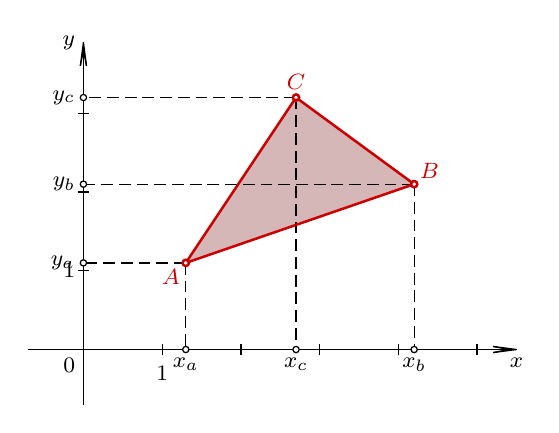
\begin{tikzpicture}
                        % \clip (0,0) rectangle (14.000000,10.000000);
                        {\footnotesize
                        
                        % Drawing 2D Cartesian system
                        \draw (2.000000,2.000000) node [anchor=north east] { $0$ };%
                        \draw [line width=0.016cm] (2.000000,1.925000) -- (2.000000,2.075000);%
                        \draw (3.000000,1.900000) node [anchor=north] { $1$ };%
                        \draw [line width=0.016cm] (3.000000,1.925000) -- (3.000000,2.075000);%
                        % \draw (4.000000,2.000000) node [anchor=north] { $2$ };%
                        \draw [line width=0.016cm] (4.000000,1.925000) -- (4.000000,2.075000);%
                        % \draw (5.000000,2.000000) node [anchor=north] { $3$ };%
                        \draw [line width=0.016cm] (5.000000,1.925000) -- (5.000000,2.075000);%
                        % \draw (6.000000,2.000000) node [anchor=north] { $4$ };%
                        \draw [line width=0.016cm] (6.000000,1.925000) -- (6.000000,2.075000);%
                        % \draw (7.000000,2.000000) node [anchor=north] { $5$ };%
                        \draw [line width=0.016cm] (7.000000,1.925000) -- (7.000000,2.075000);%
                        \draw (2.000000,3.000000) node [anchor=east] { $1$ };%
                        \draw [line width=0.016cm] (1.925000,3.000000) -- (2.075000,3.000000);%
                        % \draw (2.000000,4.000000) node [anchor=east] { $2$ };%
                        \draw [line width=0.016cm] (1.925000,4.000000) -- (2.075000,4.000000);%
                        % \draw (2.000000,5.000000) node [anchor=east] { $3$ };%
                        \draw [line width=0.016cm] (1.925000,5.000000) -- (2.075000,5.000000);%
                        \draw (7.500000,2.000000) node [anchor=north] { $x$ };%
                        \draw (2.000000,5.900000) node [anchor=east] { $y$ };%
                        \draw [line width=0.016cm] (1.300000,2.000000) -- (3.260000,2.000000);%
                        \draw [line width=0.016cm] (3.340000,2.000000) -- (4.660000,2.000000);%
                        \draw [line width=0.016cm] (4.740000,2.000000) -- (6.160000,2.000000);%
                        \draw [line width=0.016cm] (6.240000,2.000000) -- (7.500000,2.000000);%
                        \draw [line width=0.016cm] (7.202567,2.039158) -- (7.500000,2.000000);%
                        \draw [line width=0.016cm] (7.202567,2.039158) -- (7.400000,2.000000);%
                        \draw [line width=0.016cm] (7.202567,1.960842) -- (7.500000,2.000000);%
                        \draw [line width=0.016cm] (7.202567,1.960842) -- (7.400000,2.000000);%
                        \draw [line width=0.016cm] (2.000000,1.300000) -- (2.000000,3.060000);%
                        \draw [line width=0.016cm] (2.000000,3.140000) -- (2.000000,4.060000);%
                        \draw [line width=0.016cm] (2.000000,4.140000) -- (2.000000,5.160000);%
                        \draw [line width=0.016cm] (2.000000,5.240000) -- (2.000000,5.900000);%
                        \draw [line width=0.016cm] (1.960842,5.602567) -- (2.000000,5.900000);%
                        \draw [line width=0.016cm] (1.960842,5.602567) -- (2.000000,5.800000);%
                        \draw [line width=0.016cm] (2.039158,5.602567) -- (2.000000,5.900000);%
                        \draw [line width=0.016cm] (2.039158,5.602567) -- (2.000000,5.800000);%
                        
                        % Changing color 213 183 183
                        \definecolor{r213g183b183}{rgb}{0.835294,0.717647,0.717647}%
                        \color{r213g183b183}% 
                        
                        % Filling triangle A B C
                        \fill (3.300000,3.100000) -- (6.200000,4.100000) -- (4.700000,5.200000);%
                        
                        % Changing color 0 0 0
                        \definecolor{r0g0b0}{rgb}{0.000000,0.000000,0.000000}%
                        \color{r0g0b0}% 
                        
                        % Drawing segment A x_a
                        \draw [line width=0.016cm] (3.300000,3.060000) -- (3.300000,2.950000);%
                        \draw [line width=0.016cm] (3.300000,2.875000) -- (3.300000,2.725000);%
                        \draw [line width=0.016cm] (3.300000,2.650000) -- (3.300000,2.500000);%
                        \draw [line width=0.016cm] (3.300000,2.425000) -- (3.300000,2.275000);%
                        \draw [line width=0.016cm] (3.300000,2.200000) -- (3.300000,2.050000);%
                        
                        % Drawing segment A y_a
                        \draw [line width=0.016cm] (3.260000,3.100000) -- (3.150000,3.100000);%
                        \draw [line width=0.016cm] (3.075000,3.100000) -- (2.925000,3.100000);%
                        \draw [line width=0.016cm] (2.850000,3.100000) -- (2.700000,3.100000);%
                        \draw [line width=0.016cm] (2.625000,3.100000) -- (2.475000,3.100000);%
                        \draw [line width=0.016cm] (2.400000,3.100000) -- (2.250000,3.100000);%
                        \draw [line width=0.016cm] (2.175000,3.100000) -- (2.040000,3.100000);%
                        
                        % Drawing segment B x_b
                        \draw [line width=0.016cm] (6.200000,4.060000) -- (6.200000,3.950000);%
                        \draw [line width=0.016cm] (6.200000,3.875000) -- (6.200000,3.725000);%
                        \draw [line width=0.016cm] (6.200000,3.650000) -- (6.200000,3.500000);%
                        \draw [line width=0.016cm] (6.200000,3.425000) -- (6.200000,3.275000);%
                        \draw [line width=0.016cm] (6.200000,3.200000) -- (6.200000,3.050000);%
                        \draw [line width=0.016cm] (6.200000,2.975000) -- (6.200000,2.825000);%
                        \draw [line width=0.016cm] (6.200000,2.750000) -- (6.200000,2.600000);%
                        \draw [line width=0.016cm] (6.200000,2.525000) -- (6.200000,2.375000);%
                        \draw [line width=0.016cm] (6.200000,2.300000) -- (6.200000,2.150000);%
                        \draw [line width=0.016cm] (6.200000,2.075000) -- (6.200000,2.040000);%
                        
                        % Drawing segment B y_b
                        \draw [line width=0.016cm] (6.160000,4.100000) -- (6.050000,4.100000);%
                        \draw [line width=0.016cm] (5.975000,4.100000) -- (5.825000,4.100000);%
                        \draw [line width=0.016cm] (5.750000,4.100000) -- (5.600000,4.100000);%
                        \draw [line width=0.016cm] (5.525000,4.100000) -- (5.375000,4.100000);%
                        \draw [line width=0.016cm] (5.300000,4.100000) -- (5.150000,4.100000);%
                        \draw [line width=0.016cm] (5.075000,4.100000) -- (4.925000,4.100000);%
                        \draw [line width=0.016cm] (4.850000,4.100000) -- (4.700000,4.100000);%
                        \draw [line width=0.016cm] (4.625000,4.100000) -- (4.475000,4.100000);%
                        \draw [line width=0.016cm] (4.400000,4.100000) -- (4.250000,4.100000);%
                        \draw [line width=0.016cm] (4.175000,4.100000) -- (4.025000,4.100000);%
                        \draw [line width=0.016cm] (3.950000,4.100000) -- (3.800000,4.100000);%
                        \draw [line width=0.016cm] (3.725000,4.100000) -- (3.575000,4.100000);%
                        \draw [line width=0.016cm] (3.500000,4.100000) -- (3.350000,4.100000);%
                        \draw [line width=0.016cm] (3.275000,4.100000) -- (3.125000,4.100000);%
                        \draw [line width=0.016cm] (3.050000,4.100000) -- (2.900000,4.100000);%
                        \draw [line width=0.016cm] (2.825000,4.100000) -- (2.675000,4.100000);%
                        \draw [line width=0.016cm] (2.600000,4.100000) -- (2.450000,4.100000);%
                        \draw [line width=0.016cm] (2.375000,4.100000) -- (2.225000,4.100000);%
                        \draw [line width=0.016cm] (2.150000,4.100000) -- (2.040000,4.100000);%
                        
                        % Drawing segment C x_c
                        \draw [line width=0.016cm] (4.700000,5.160000) -- (4.700000,5.050000);%
                        \draw [line width=0.016cm] (4.700000,4.975000) -- (4.700000,4.825000);%
                        \draw [line width=0.016cm] (4.700000,4.750000) -- (4.700000,4.600000);%
                        \draw [line width=0.016cm] (4.700000,4.525000) -- (4.700000,4.375000);%
                        \draw [line width=0.016cm] (4.700000,4.300000) -- (4.700000,4.150000);%
                        \draw [line width=0.016cm] (4.700000,4.075000) -- (4.700000,3.925000);%
                        \draw [line width=0.016cm] (4.700000,3.850000) -- (4.700000,3.700000);%
                        \draw [line width=0.016cm] (4.700000,3.625000) -- (4.700000,3.475000);%
                        \draw [line width=0.016cm] (4.700000,3.400000) -- (4.700000,3.250000);%
                        \draw [line width=0.016cm] (4.700000,3.175000) -- (4.700000,3.025000);%
                        \draw [line width=0.016cm] (4.700000,2.950000) -- (4.700000,2.800000);%
                        \draw [line width=0.016cm] (4.700000,2.725000) -- (4.700000,2.575000);%
                        \draw [line width=0.016cm] (4.700000,2.500000) -- (4.700000,2.350000);%
                        \draw [line width=0.016cm] (4.700000,2.275000) -- (4.700000,2.125000);%
                        \draw [line width=0.016cm] (4.700000,2.050000) -- (4.700000,2.040000);%
                        
                        % Drawing segment C y_c
                        \draw [line width=0.016cm] (4.660000,5.200000) -- (4.550000,5.200000);%
                        \draw [line width=0.016cm] (4.475000,5.200000) -- (4.325000,5.200000);%
                        \draw [line width=0.016cm] (4.250000,5.200000) -- (4.100000,5.200000);%
                        \draw [line width=0.016cm] (4.025000,5.200000) -- (3.875000,5.200000);%
                        \draw [line width=0.016cm] (3.800000,5.200000) -- (3.650000,5.200000);%
                        \draw [line width=0.016cm] (3.575000,5.200000) -- (3.425000,5.200000);%
                        \draw [line width=0.016cm] (3.350000,5.200000) -- (3.200000,5.200000);%
                        \draw [line width=0.016cm] (3.125000,5.200000) -- (2.975000,5.200000);%
                        \draw [line width=0.016cm] (2.900000,5.200000) -- (2.750000,5.200000);%
                        \draw [line width=0.016cm] (2.675000,5.200000) -- (2.525000,5.200000);%
                        \draw [line width=0.016cm] (2.450000,5.200000) -- (2.300000,5.200000);%
                        \draw [line width=0.016cm] (2.225000,5.200000) -- (2.075000,5.200000);%
                        
                        % Marking point x_a by circle
                        \draw [line width=0.016cm] (3.300000,2.000000) circle (0.040000);%
                        \draw (3.300000,2.000000) node [anchor=north] { $x_a$ };%
                        
                        % Marking point x_b by circle
                        \draw [line width=0.016cm] (6.200000,2.000000) circle (0.040000);%
                        \draw (6.200000,2.000000) node [anchor=north] { $x_b$ };%
                        
                        % Marking point y_a by circle
                        \draw [line width=0.016cm] (2.000000,3.100000) circle (0.040000);%
                        \draw (2.000000,3.100000) node [anchor=east] { $y_a$ };%
                        
                        % Marking point y_b by circle
                        \draw [line width=0.016cm] (2.000000,4.100000) circle (0.040000);%
                        \draw (2.000000,4.100000) node [anchor=east] { $y_b$ };%
                        
                        % Marking point x_c by circle
                        \draw [line width=0.016cm] (4.700000,2.000000) circle (0.040000);%
                        \draw (4.700000,2.000000) node [anchor=north] { $x_c$ };%
                        
                        % Marking point y_c by circle
                        \draw [line width=0.016cm] (2.000000,5.200000) circle (0.040000);%
                        \draw (2.000000,5.200000) node [anchor=east] { $y_c$ };%
                        
                        % Changing color 204 0 0
                        \definecolor{r204g0b0}{rgb}{0.800000,0.000000,0.000000}%
                        \color{r204g0b0}% 
                        
                        % Drawing segment A B
                        \draw [line width=0.032cm] (3.337815,3.113040) -- (6.162185,4.086960);%
                        
                        % Drawing segment C B
                        \draw [line width=0.032cm] (4.732256,5.176345) -- (6.167744,4.123655);%
                        
                        % Drawing segment A C
                        \draw [line width=0.032cm] (3.322188,3.133282) -- (4.677812,5.166718);%
                        
                        % Marking point A by circle
                        \draw [line width=0.032cm] (3.300000,3.100000) circle (0.040000);%
                        \draw (3.330000,3.130000) node [anchor=north east] { $A$ };%
                        
                        % Marking point B by circle
                        \draw [line width=0.032cm] (6.200000,4.100000) circle (0.040000);%
                        \draw (6.170000,4.070000) node [anchor=south west] { $B$ };%
                        
                        % Marking point C by circle
                        \draw [line width=0.032cm] (4.700000,5.200000) circle (0.040000);%
                        \draw (4.700000,5.200000) node [anchor=south] { $C$ };%
                        \color{black}
                        }
                        \end{tikzpicture}
                        
                \end{block}}
            \end{columns}

        \end{frame}



        %%% naloge

        \begin{frame}

            \only<2->{\begin{exampleblock}{Naloga}
                Narišite trikotnik $\triangle ABC$ in izračunajte njegovo ploščino.
                \begin{itemize}
                    \item $A(-4,-2)$, $B(5,1)$ in $C(-2,5)$ \\~
                    \item $A(2,1)$, $B(-5,1)$ in $C(2,6)$ \\~
                \end{itemize}
            \end{exampleblock}}

            \only<3->{\begin{exampleblock}{Naloga}
                Ali so točke kolinearne?
                \begin{itemize}
                    \item $P(-4,-5)$, $Q(4,-1)$ in $R(10,2)$ \\~
                    \item $X(1,-7)$, $Y(-2,2)$ in $Z(3,2)$ \\~
                \end{itemize}
            \end{exampleblock}}

        \end{frame}


        \begin{frame}

            \only<2->{\begin{exampleblock}{Naloga}
                Določite $x$ tako, da bo trikotnik $\triangle ABC$, z oglišči v $A(-2,-3)$, $B(5,3)$ in $C(x,-1)$ negativno orientiran 
                in bo imel ploščino $17$. \\~
            \end{exampleblock}}
           
            \only<3->{\begin{exampleblock}{Naloga}
                Določite $p$ tako, da bo imel trikotnik $\triangle ABC$, z oglišči v $A(2,3)$, $B(p,-3)$ in $C(-1,6)$, ploščino $18$. \\~
            \end{exampleblock}}

            \only<4->{\begin{exampleblock}{Naloga}
                Dani sta točki $A(2,-4)$ in $B(8,3)$. Določite koordinati točke $C$, ki leži na simetrali lihih kvadrantov, 
                da bo trikotnik $\triangle ABC$ pozitivno orientiran in bo imel ploščino $17$. \\~
            \end{exampleblock}}


        \end{frame}

